\documentclass[a4paper,11pt]{book}
\usepackage{import}
\usepackage{style}
\usepackage{makeidx}
%\includeonly{Cap1-Probabilidad/section1-4}
\includeonly{Cap5-AnálisisEsquitosoma/section5-1}
%\includeonly{Cap3-ProcesosEstocásticos/section3-1}
%\includeonly{Cap4-EDP/section4-0}
\makeindex
\begin{document}
\frontmatter
\import{./}{title.tex}

\clearpage
\thispagestyle{empty}

\tableofcontents

\mainmatter
\chapter{Introducción a la teoría de la probabilidad}
    Este capítulo pretende presentar una introducción a la formulación moderna de la Teoría de la Probabilidad que serán utilizados en la formulación de nuestra ecuación, intentando buscar la motivación tratando de buscar el origen de ellos.\\\\
    La teoría de la probabilidad ha resultado muy útil para modelar
    matemáticamente fenómenos de diversas disciplinas en donde es necesario incorporar el azar como elemento esencial del modelo. Así, la probabilidad puede definirse como
    aquella rama de las matemáticas que se encarga del estudio de los fenómenos
    aleatorios.
    
    \section{Conceptos generales}
    En la naturaleza se pueden encuentran dos tipos de fenómenos o experimentos: deterministas y aleatorios. Un experimento determinista es aquel cuyo resultado es el mismo si se la repite bajo las mismas condiciones, como por ejemplo, el medir el volumen de un gas en teoría produce siempre el mismo resultado, cuando la presión y la temperatura son constantes.\\
    En contraste a esto, un experimento aleatorio es aquel que aunque se repitan bajo las mismas condiciones, el resultado no será siempre el mismo.\\
    Los conceptos y teoremas expuestos en esta sección fueron tomados de \cite{Rincon1} \cite{Rincon2}.
\begin{Ejm}
    Algunos ejemplos de experimentos deterministas:
    \begin{enumerate}[a)]
        \item Medir el volumen de un gas cuando la presión y la temperatura son constantes.
        \item Calcular la distancia que recorre un carro en $1$ hora a una velocidad constante.
    \end{enumerate}
\end{Ejm}
\begin{Ejm}
\label{Prob-Ejm-Aleatorio}
Algunos ejemplos de experimentos aleatorios:
    \begin{enumerate}[a)]
        \item Registrar el número de accidentes que ocurren en una determinada calle de una ciudad.
        \item Registrar si una mujer con  determinada enfermedad la trasmite a alguno de sus 3 hijos.
    \end{enumerate}
\end{Ejm}
Cuando se tratan de experimentos aleatorios, en principio no sabremos cuál será el resultado obtenido. El experimento asociado a nuestro fenómeno, da lugar a un solo resultado (que denotaremos $\omega$) de entre un conjunto de posibles resultados.
\begin{Def}
Un espacio muestral es un conjunto arbitrario $\Omega$ que tiene como objetivo agrupar todos los posibles resultados del experimento aleatorio en cuestión.
\end{Def}
\begin{Ejm}
Los espacios muestrales respecto a los experimentos aleatorios descritos en el ejemplo (\ref{Prob-Ejm-Aleatorio}) serían:
\begin{enumerate}[a)]
    \item $\Omega=\{0,1,2,3,\ldots\}$
    \item $\Omega=\{\textit{true, false}\}$
\end{enumerate}
\end{Ejm}
De manera intuitiva, los subconjuntos de resultados (es decir del conjunto $\Omega$) que comparten alguna característica en común reciben el nombre de sucesos aleatorios.
Estos subconjuntos recibirán los nombres de sucesos si cumplen determinadas condiciones. Cuando el resultado de un experimento realizado pertenece a un suceso específico $A$, decimos que "$A$ ha ocurrido o se ha realizado".
\begin{Def}
    Una clase o colección $\mathscr{F}$ de subconjuntos de $\Omega$ es un $\sigma- \textit{álgebra}$ si cumple que:
    \begin{enumerate}
        \item $\Omega\in\mathscr{F}$
        \item Si $A\in\mathscr{F}$ entonces $A^c\in\mathscr{F}$
        \item Si $\{A_n\}_{n\in\N}\in\mathscr{F}$, entonces  $\bigcup_{k=1}^\infty A_k\in\mathscr{F}$
    \end{enumerate}
\end{Def}
 Formalmente, a los elementos de un $\sigma-$álgebra $\mathscr{F}$ se los llama eventos, sucesos aleatorios o conjuntos medibles.
 Veamos un ejemplo que nos ayuda a ver intuitivamente el concepto de $\sigma-$álgebra.
\begin{Ejm}
    Supongamos que queremos registrar el número final de las placas de los carros que circulan en una determinada calle de una ciudad, para poder aplicar la regla de pico y placa. Para este caso, el espacio muestral de todos los posibles números finales de una placa arbitraria serían 
    $$\Omega=\{0,\thinspace 1,\thinspace 2,\ldots 9\}.$$
    Sea $\omega$ es resultado del experimento, sea cual su valor, $\omega \in\Omega$, por tanto, $\Omega$ debe ser un evento; al cual llamaremos evento seguro. Esto es $\Omega\in\mathscr{F}.$\\ Definamos el evento $A=\{0,\thinspace 2,\ldots ,8\}.$ Esto se interpreta al suceso de que la placa del auto arbitrario termine en número par. Si tiene perfecto sentido pensar en que el resultado $\omega$ pueda ser un número par (es decir $\omega\in A$), también tiene perfecto sentido pensar que este podría ser un número impar (es decir que $\omega \in A^c$) es, por tanto, razonable exigir que $A^c$ sea un evento si $A$ lo es. Esto es $A^c\in\mathscr{F}$ si $A\in\mathscr{F}.$\\Si definimos el evento $B=\{1\}$ que ocurre cuando la placa acabe en el número $1$, tiene sentido pensar que escogiendo un auto arbitrario, el resultado $\omega$ podría ser un par ($\omega\in A$) o quizá el resultado podría ser $1$ ($\omega\in B$). Por ser ambos eventos, puede ocurrir que $\omega\in A\cup B$, por lo tanto exigiremos que la unión finita de sucesos sea un suceso. Esto es si $A,\thinspace B\in\mathscr{F}$ entonces $A\cup B\in \mathscr{F}.$
\end{Ejm}
Menos intuitiva es la exigencia de estabilidad frente a uniones numerables, la respuesta más
convincente es que, de ese modo, se obtiene una teoría matemática más rica.
\begin{Def}
    Si $\mathscr{C}$ es una colección no vacía de subconjuntos de $\Omega$.\\La $\sigma-\textit{álgebra}$ generada por $\mathscr{C}$ denotada por $\sigma(\mathscr{C})$ es $$\sigma(\mathscr{C})=\bigcap\{\mathscr{F}|\thinspace\mathscr{F} \textit{ es un }\sigma-\textit{álgebra y }  \mathscr{C}\subset\mathscr{F}\}$$
    Este conjunto es la menor $\sigma-$álgebra que contiene a $\mathscr{C}$.
\end{Def}
\begin{Ejm}
    El conjunto $\mathscr{P}(\Omega)$ de todos los subconjuntos de $\Omega$ es trivialmente un $\sigma$-álgebra en $\Omega$ a la cual llamaremos discreta. \\ Llamaremos espacio medible discreto a un conjunto numerable provisto de esta $\sigma-$álgebra. En lo que sigue, cualquier conjunto numerable se supondrá provisto de la $\sigma-$álgebra discreta, a menos que se indique lo contrario.
\end{Ejm}
\begin{Ejm}
    El conjunto $\{\Omega, \emptyset\}$ es la más pequeña $\sigma-$álgebra que podemos considerar de $\Omega$. Se llamará $\sigma-$álgebra trivial.
\end{Ejm}
\begin{Def}
    \label{def-medidaProbabilidad}
    Sea $\mathscr{F}$ una $\sigma-$álgebra del espacio muestral $\Omega$, $k\in\N$ $A_k$, sucesos asociados a $\mathscr{F}$.
    Una función $P:\mathscr{F}\rightarrow [0,1]$ es una medida de probabilidad si cumple que $P(\Omega)=1$ y P es $\sigma-aditiva$, es decir que se cumple que $$P\big(\bigcup_{k=1}^\infty A_k\big)=\sum_{k=1}^\infty P(A_k)$$
    donde $A_i\cap A_j=\emptyset$, para $i\not= j$
\end{Def}
El número $P(A)$ es una forma de medir la posibilidad que suceda el evento $A$ al efectuar una vez el experimento aleatorio.\\
Una probabilidad cercana a $0$ indica que es poco probable que ocurra un evento, mientras que una probabilidad cercana a $1$ indica que es casi seguro que éste ocurra.\\
La probabilidad es importante en la toma de decisiones debido a que proporciona una manera de medir, expresar y analizar las incertidumbres asociadas con eventos futuros.
\begin{Def}
    Sea $\Omega$ un espacio muestral, $\mathscr{F}$ un $\sigma-$álgebra de $\Omega$, $P$ una medida de probabilidad.\\
    A la terna $(\Omega,\thinspace\mathscr{F})$ se le llama espacio de medida o espacio medible y a la terna $(\Omega,\mathscr{F},P)$ se le conoce como espacio de probabilidad.
\end{Def}
    \section{Algunas propiedades elementales}

La importancia esencial de la aplicación de los métodos de cálculo de la probabilidad reside en su capacidad para estimar o predecir eventos. Cuanto mayor sea la cantidad de datos disponibles para calcular la probabilidad de un acontecimiento, más preciso será el resultado calculado. Dada la complejidad de los sistemas en los que suele aplicarse la teoría de la probabilidad, se requiere de ciertas propiedades que faciliten su cálculo.
Las demostraciones de los resultados expuestos en este capítulo se pueden encontrar en \cite{intro-probabilidad}, \cite{Feller},\cite{Rincon1} \cite{Rincon2}
\begin{Prop}
    Sea $(\Omega,\thinspace\mathscr{F},P)$ un espacio de probabilidad; $A,B\subset\Omega$ se cumple que:
    \begin{enumerate}
        \item $P(A^c)=1-P(A)$.
        \item $P(\emptyset)=0$.
        \item Si $A\subseteq B$ entonces $P(A)\leq P(B)$.
        \item Si $A\subseteq B$ entonces $P(B-A)=P(B)-P(A)$.
    \end{enumerate}
\end{Prop}
\begin{Def}
    Sea $\Omega$ el espacio muestral de un experimento aleatorio. Decimos que la colección de eventos $\{B_1,B_2,\ldots,B_n\}$ es una partición finita de $\Omega$ si se cumplen las siguientes condiciones:
    \begin{enumerate}[a)]
        \item $B_i\subset\Omega$ $i=1,2,\ldots,n$.
        \item $B_i\not=\emptyset$, $i=1,2,\ldots,n$.
        \item $B_i\cap B_j=\emptyset$ , para $i\not= j$.
        \item $\bigcup_{i=1}^n B_i=\Omega$.
    \end{enumerate}
\end{Def}
El siguiente resultado es bastante útil, pues establece un método para calcular las probabilidades. Mediante este método, dado un evento $A$ cuya probabilidad se busca, se trata de encontrar una partición de $A$ donde cada evento de esta partición será más simple de calcular.
\begin{Prop}
    Sea $(\Omega,\mathscr{F},P)$ un espacio de probabilidad, $\{A_k\}_{k=1}^n$ una partición finita de $\Omega$, se tiene que
    $$P(\bigcup_{k=1}^n A_k)=\sum_{k=1}^n P(A_k)$$ 
\end{Prop}
\begin{Cor}
    Si $(\Omega,\mathscr{F},P)$ es un espacio de probabilidad, $A$ y $B$ eventos, entonces
    $$P(A\cup B)=P(A)+P(B)-P(A\cap B)$$
\end{Cor}
En algunos casos, nos topamos con una colección de eventos que tienen cada uno la misma probabilidad de que sucedan. A estos eventos se llaman equiprobables.
Dado $n,N\in\N$, tal que $n<N$, $\Omega=\{\omega_1,\ldots,\omega_N\}$ un espacio muestral y $A=\{\omega_1,\ldots,\omega_n\}$ un evento del espacio muestral $\Omega$.
Si suponemos que los conjuntos  $\{\omega_k\}_{k=1}^N$, son equiprobables, entonces $P(\{\omega_i\})=P(\{\omega_j\})$ para $i,j=1,2,\ldots,N$, $i\not=j$ y como consecuencia $$1=P(\bigcup_{k=1}^N \{\omega_k\})=\sum_{k=1}^N P(\{\omega_k\})=N P(\omega_k).$$
\begin{eqnarray}
    \label{probabilidadn}
    P(\omega_k)=\frac{1}{N}\quad k=1,2,\ldots ,N.
\end{eqnarray}
Además
$$P(A)=P(\bigcup_{k=1}^n \{\omega_k\})=\sum_{k=1}^n P(\{\omega_k\})=n P(\{\omega_k\})$$
Usando la expresión (\ref{probabilidadn})
$$P(A)=\frac{n}{N}.$$
Este método de encontrar probabilidades, basándose en la equiprobabilidad de los posibles resultados, es conocido como la definición clásica de probabilidad.\\
Históricamente,esta forma de calcular probabilidades es una de las primeras en utilizarse; se aplicó con bastante éxito en problemas de juegos de azar y ayudó a sentar las bases para construir la teoría matemática.
\begin{Def}
    Sea $A$ un subconjunto de un espacio muestral $\Omega$ de cardinalidad finita. Si $\#A$ denota la cardinalidad del conjunto $A$. Se define la probabilidad clásica del evento $A$ como el cociente $$P(A)=\frac{\#A}{\#\Omega}$$
    \label{defprobClásica}
\end{Def}
\begin{Ejm}
    El ejemplo típico de equiprobabilidad se presenta al considerar el experimento  en lanzar un dado no trucado sobre una mesa y observar el número que muestra finalmente su cara superior. Considere el experimento aleatorio de lanzar un dado equilibrado.\\ El espacio muestral es el conjunto  $\Omega=\{1,\thinspace 2\thinspace 3,\thinspace 4,\thinspace 5,\thinspace 6\}$. Si deseamos calcular la probabilidad (clásica) del evento A, correspondiente a obtener un número par, es decir, la probabilidad de $A=\{2,\thinspace 4,\thinspace 6\}$, entonces $$P(A)=\frac{\#\{2,\thinspace 4,\thinspace 6\}}{\#\{1,\thinspace 2\thinspace 3,\thinspace 4,\thinspace 5,\thinspace 6\}}=\frac{3}{6}=0.5$$
\end{Ejm}
En ocasiones un experimento aleatorio depende de otros experimentos, también aleatorios, los cuales se realizan uno después del otro.\\
Como la probabilidad está ligada a nuestra ignorancia sobre los resultados de la experiencia, el hecho de que ocurra un suceso, puede cambiar la probabilidad de los demás.
\begin{Def}
    Sea $(\Omega,\mathscr{F},P)$ un espacio de probabilidad, $A,B\subset\Omega$ tal que $P(B)>0$. La probabilidad condicional de algún evento $A$, dado que el evento $B$ suceda previamente, es una función que se denota $P(\cdot\thinspace|\thinspace B):\Omega\rightarrow [0,1]$ y se define como $$P(A\thinspace|\thinspace B)=\frac{P(A\cap B)}{P(B)}$$
\end{Def}
Cuando ocurre un suceso antes de realizar otro experimento, se reduce el espacio muestral y es por eso que cambia la probabilidad. A veces es más fácil calcular la probabilidad condicionada teniendo en cuenta este cambio de espacio muestral.
No tiene por qué haber una relación causal o temporal entre $A$ y $B$. A puede preceder en el tiempo a $B$, sucederlo o pueden ocurrir simultáneamente. $A$ puede causar $B$, viceversa o pueden no tener relación causal. Las relaciones causales o temporales son nociones que no pertenecen al ámbito de la probabilidad. Pueden desempeñar un papel o no, dependiendo de la interpretación que se le dé a los eventos.
Siendo la probabilidad condicional una probabilidad calculada en un espacio muestral reducido (el cual sería $B$), es de esperarse que ésta tenga las mismas propiedades que cualquier medida de probabilidad.
\begin{Ejm}
Se piensa tomar dos exámenes, uno de álgebra y otro de cálculo.
Si 6 de cada 10 alumnos aprueban el examen de álgebra, mientras que solo 1 de cada 4 alumnos  álgebra y cálculo a la vez. Si el examen de álgebra se toma primero. ¿Cuál es la probabilidad que un alumno luego de aprobar álgebra también apruebe cálculo?
    Vamos a trabajar con 2 eventos: que el alumno apruebe cálculo, y que apruebe álgebra.\\
    Evento A: Aprobar cálculo. $P(A) = ?$\\
    Evento B: Aprobar álgebra. $P(B) =0.6$ .\\
    Evento A y B: Aprobar álgebra y cálculo. $P(A\cap B) =0.25$\\
    Ahora calculamos la probabilidad que un alumno luego de aprobar álgebra también apruebe cálculo
    $$P(A\thinspace|\thinspace B)=\frac{P(A\cap B)}{P(B)}=\frac{0.25}{0.6}=0.4167$$
  Como vemos, luego de tomar el examen de álgebra el espacio muestral ($100\%$ de la los alumnos) se reduce al evento $B$ ( los que aprueban álgebra, $60 \%$ de la totalidad de los alumnos).
  \end{Ejm}
\begin{Prop}
    $P(\cdot\thinspace|\thinspace B)$ es una medida de probabilidad en el espacio de medida $(\Omega,\mathscr{F})$
\end{Prop}
Gracias a esta propiedad tenemos una útil herramienta para calcular probabilidades conocida como la regla del producto, la cual se puede utilizar para determinar la probabilidad de la intersección de dos eventos. Esta ley se deriva de la definición de probabilidad condicional.
$$P(A\cap B)=P(A\thinspace|\thinspace B)P(B)$$
De la misma manera, en los casos en que la ocurrencia de un evento $A$ no altere la probabilidad de otro evento $B$, se puede hablar de independencia de probabilidad.
\begin{Def}
    Se dice que los eventos $A, B$ son independientes si se cumple la igualdad $P(A\cap B)=P(A)P(B)$. Bajo la hipótesis adicional que $P(B)>0$ la condición de independencia puede escribirse como $P(A\thinspace|\thinspace B)=P(A)$.
\end{Def}
 Esto intuitivamente significa que la ocurrencia del evento $B$ no afecta al evento $A$.
El siguiente resultado es bastante útil cuando se quiere determinar la probabilidad de algún conjunto grande, bastará con hallar las probabilidades de conjuntos más pequeños y probabilidades condicionales con respecto a esos conjuntos
\begin{Teo}
    Sea $\{B_1,B_2,\ldots,B_n\}$ una partición de $\Omega$ tal que $P(B_i)\not=0$, para  $i=1,\ldots,n$, para cualquier evento $A$, $$P(A)=\sum_{i=1}^n P(A\thinspace|\thinspace B_i)P(B_i)$$
\end{Teo}


    \section{Variables aleatorias}
En ocasiones, dado un experimento aleatorio, estamos interesados en alguna característica numérica del resultado que se obtiene. Por ejemplo, al considerar el lanzamiento de un par de dados, pudiéramos estar interesados no en el resultado específico que se obtiene con cada dado, sino en la suma de ellos.\\
Nuestra primera dificultad es que no todos los espacios muestrales $\Omega$ son subconjuntos de $\R$, por ello, es necesario introducir la definición de una función que traslade los elementos de $\Omega$ a números reales con los cuales podamos trabajar matemáticamente.\\
Las demostraciones de los resultados expuestos en este capítulo se pueden encontrar en \cite{intro-probabilidad}, \cite{Feller},\cite{Rincon1} \cite{Rincon2}
%%%%%%%%%%%%%%%%%%%%%%%%%%%%%%%%%%%%
\begin{comment}
\begin{Def}
El $\sigma-$álgebra de Borel en $\R$ denotado por $\mathscr{B}(\R)$ es
$$\mathscr{B}(\R)=\sigma(\{(a,\thinspace b)\subset\R:a\leq b\})$$
\end{Def}
\begin{Prop}
\textbf{ }\\
\begin{enumerate}
    \item Todo intervalo de $\R$ es un booreliano.
    \item Los subconjuntos cerrados y abiertos de $\R$ son borelianos
\end{enumerate}
\end{Prop}
\begin{Def}
Una función $\phi:\R^n\rightarrow\R^m$ es llamada boreliana si $\phi^{-1}(B)$ es un conjunto boreliano de $R^{-1}$ para todo boreliano B de $\R$.
\end{Def}
Recuérdese que si $\phi:\R^n\rightarrow\R^m$ es cualquier función, se cumple que $\phi^{-1}(B^c)=[\phi^{-1}(B)]^c$
 $\phi^{-1}(\bigcup_{\lambda}B_{\lambda})=\bigcup_{\lambda}\phi^{-1}(B_\lambda)$. Esto
implica que $\{B\subset \R^m: \phi^{-1}(B)\in B(\R^n)\}$ es un $\sigma$-álgebra de subconjuntos de $R^m$ , de manera que, para demostrar que una
cierta función f es boreliana, basta con probar que $\phi^{-1}(B)$ es un conjunto boreliano de $\R^n$ para cualquier elemento B abierto (o cualquier elemento B de una familia de generadores de los borelianos de $\R^m$).
Con base de esta idea, se pueden demostrar las siguientes proposiciones.
\begin{Prop}
$\phi:\R^n\rightarrow\R^m$,  $g:\R^m\rightarrow\R^p$ son borelianos, entonces $g\circ\phi$ es boreliano
\end{Prop}
\begin{Prop} Si $\phi:\R^n\rightarrow\R^m$ es continua, entonces es boreliana.
\end{Prop}
\end{comment}
%%%%%%%%%%%%%%%%%%%%%%%%%%%%%%%%%%
\begin{Def}
    Sean $(\Omega_1,\mathscr{F}_1)$, $(\Omega_2,\mathscr{F}_2)$ espacios medibles. Una variable aleatoria (llamado función medible en teoría de la medida) es una función $X:\Omega_1\rightarrow \Omega_2$ tal que para cualquier $F\in\mathscr{F}_2$ se cumple que $$X^{-1}(F)\in\mathscr{F}_1.$$
\end{Def}
 Al conjunto $X(\Omega_1)$ se le conocerá como el conjunto de estados de X.
\begin{Obs}
    Si el conjunto de estados $X(\Omega_1)$ es numerable o finito, entonces $X$ será llamado una variable aleatoria discreta.
\end{Obs}
\begin{Ejm}
  Se tiene un experimento aleatorio que consiste en lanzar 2 dados, cuyo  espacio muestral será $$\Omega_1=\{(1,1),\ldots,(1,6),\thinspace(2,1),\ldots\ldots,(2,6),\ldots,(6,6)\}$$y $\sigma-$álgebra asociado $\mathscr{P}(\Omega)$.\\ 
   Si queremos obtener la diferencia entre el mayor y el menor de los números que se obtienen al lanzar los dos dados, se define a la variable aleatoria $X$ como $X:\Omega_1\rightarrow \{0,\thinspace 1,\ldots\}$ $X(a,b)=\max \{a,b\}-\min\{a,b\}$
\end{Ejm}
Si $(\Omega_1,\mathscr{F},P)$ es un espacio de probabilidad, gracias a a la variable aleatoria $X$ se puede definir una nueva medida de probabilidad $P_X$ sobre el espacio de medida $(\Omega_2,\mathscr{F}_2)$, definida como $P_X(F)=P(X^{-1}(F))$, ya que $X^{-1}(F)\in\mathscr{F}_1$. Además, $$P_X(\Omega_2)=P(X^{-1}(\Omega_2))=P(\Omega_1)=1$$ $$P_X\big(\bigcup_{k=1}^\infty F_k\big)=P(X^{-1}\big(\bigcup_{k=1}^\infty
F_k\big))=P \big(\bigcup_{k=1}^\infty X^{-1}(F_k) \big)=\sum_{k=1}^\infty P(X^{-1}(F_k))=\sum_{k=1}^\infty P_X(F_k)$$
de donde se concluye que $P_X(\Omega_2)= 1$ y $P_X$ es $\sigma-$aditiva.\\
De aquí se concluye que $P_X:\mathscr{F_2}\rightarrow [0,1]$ resulta ser también una medida de probabilidad, y es llamada medida de probabilidad inducida por la variable aleatoria $X$.\\
\begin{Obs}
    Para un uso más práctico , el conjunto\\ $X^{-1}(\{a\})=\{\omega\in\Omega: X(\omega)=a\}$será denotado $(X= a)$\\
\end{Obs}
Para hacer la escritura más corta, a menudo se omite el término de la variable aleatoria para $X$ suponiendo, en la mayoría de las veces que lo es, por ello escribiremos $P$ en lugar de $P_X$\\\\
Las variables aleatorias establecen una relación funcional entre elementos del espacio muestral asociado al experimento y números reales, por ello, de manera práctica, la mayoría de variables aleatorias discretas no puedan ser expresadas matemáticamente, por lo cual suelen usarse expresiones que den entender el comportamiento de la variable aleatoria. \\Algunos ejemplos de estos casos serían: $X$=\textit{"Número de fallecidos en Enero el 2020"}, $X$=\textit{"Cantidad de bacterias en determinado cultivo"}, $X$=\textit{"Número de infectados por día de determinada enfermedad"}, etc.\\
En ocasiones, los sucesos elementales de un experimento aleatorio son conjuntos de números reales, de los cuales, aparentemente no hay necesidad de usar ninguna variable aleatoria, sin embargo, en ocasiones, sí es necesario utilizarla por los múltiples usos que pueda tener.\\
Además, de un mismo experimento aleatorio se puede definir diferentes variables aleatorias.
\begin{Ejm}
    Al lanzar $3$ monedas al aire podemos asignar a cada suceso la variable aleatoria $X$=\textit{"número de caras"}, pero también se puede definir otra variable aleatoria $Y$="número de sellos". \\
    Antes que nada, vamos al construir el espacio muestral del experimento. Éste sería:
    $$\Omega = \{(C,C,C),(C,X,C), (X,C,C), (C,C,X), (X,X,C), (X,C,X), (X,X,C), (X,X,X)\}$$
Supongamos que se desea saber cuál es la probabilidad de obtener $2$ caras al lanzar las $3$ monedas.
Esto es, $$P_{X}(X=2)= P\big(X^{-1}(2)\big)= P\big(\big\{(C,X,C), (X,C,C), (C,C,X)\big\}\big)=\frac{3}{8}$$
Intuitivamente, esta probabilidad vendría a ser la misma a obtener solo un sello al lanzar las $3$ monedas.
Esto es,
$$P_{Y}(Y=1)= P\big(Y^{-1}(1)\big)= P\big(\big\{(C,X,C), (X,C,C), (C,C,X)\big\}\big)=\frac{3}{8}$$
Esto sucede ya que el conjunto $(Y=1)$ es el mismo a $(X=2)$.
\end{Ejm}
Supongamos que $(\Omega,\thinspace \mathscr{F},\thinspace P)$ es un espacio de probabilidad dado. Todas las variables aleatorias que se consideran a continuación están definidas sobre este espacio de probabilidad.
\begin{Prop}
    Si $X$ es una variable aleatoria y $c$ es una constante, entonces $c X$ también es una variable aleatoria.
    \label{prop-variableAl-cXesVA}
\end{Prop}
\begin{Prop}
    Si $X$ e $Y$ son variables aleatorias, entonces $X+Y$ es variable aleatoria
    \label{prop-variableAl-X+YesVA}
\end{Prop}
\begin{comment}
\begin{Def}
    Sea los espacios de probabilidad $(\Omega_1,\thinspace\mathscr{F}_1,\thinspace P_1)$, $(\Omega_2,\thinspace\mathscr{F}_2,\thinspace P_2)$.
    Un vector aleatorio es una función $X:\Omega_1\rightarrow\Omega_2$ tal que para cualquier conjunto B en $\mathscr{F}_2$, se cumple que la imagen inversa $X^{-1}(B)$ es un elemento de $\mathscr{F}_1$.
\end{Def}
Dado entonces que un vector aleatorio es una función de $\Omega$ en $\R^n$, éste
puede representar de la forma $X=(X_1,\ldots, X_n)$ en donde cada coordenada es una función de $\Omega$ en $\R$.
\begin{Prop}
    Una función $(X_1 , . . . , X_n):\Omega\rightarrow R^n$ es un vector aleatorio si, y sólo si, cada coordenada es una variable aleatoria.
\end{Prop}
El resultado es análogo al caso unidimensional y puede extenderse al caso de $n$ dimensiones.
En la mayoría de los casos, las definiciones y resultados son fácilmente extendidos a dimensiones mayores.\\
\begin{Obs}
    El vector aleatorio $(A,\thinspace B)$ se interpreta cuan probable es que suceda A y B a la vez. Es decir $P(A,\thinspace B)=P(A\cap B)$.
\end{Obs}
\end{comment}
\begin{Obs}
En ocasiones denotaremos a la probabilidad de que ocurran los sucesos $A$ y $B$ como $P(A,\thinspace B)$ en lugar de $P(A\cap B)$. Esto es para simplificar la notación cuando queremos expresar la probabilidad de múltiples conjuntos.
\end{Obs}
%%%%%%%%%%%%%%%%%%%%%%%%%%%%%%%%
\begin{comment}
\begin{Def}
Se dice que un conjunto $A\subset\R$ tiene medida cero si, para cualquier $\epsilon>0$, existe una colección finita o infinita numerable de intervalos abiertos $\{I_n\}$ tal que $A\subset\bigcup I_n$ y $\sum_{n} I_n<\epsilon$
\end{Def}
La familia de conjuntos borelianos, si bien es bastante grande, presenta una limitación consistente en que un conjunto de medida cero puede no ser boreliano. En un problema de probabilidad, esto a su vez se traduce en que puede haber subconjuntos de conjuntos de probabilidad
cero para los cuales, por no ser borelianos, no está definida la función de probabilidad P, y por ende, tampoco $P_X$. Esto limitaría inlcusive a la función X del cual queremos extraer un valor numérico, pues debido a esto, podría existir algún $B\in B(\R)$ tal que $X^{-1}(B)$ tenga medida cero pero no sea boreleano. Esto sigificaría que X dejaría de ser un variable aleatoria.
Por esa razón, es conveniente considerar una $\sigma-$álgebra más grande que los borelianos, que incluya a todos los conjuntos de medida cero.
\begin{Def}
Diremos que un conjunto $A \subset\R $es
Lebesgue medible si pertenece a la $\sigma$-álgebra de subconjuntos de $\R$ generada por los borelianos y los conjuntos de medida cero.
$\mathscr{L}=\sigma(\{B: B\in B(\R) \textit{ o } B \textit{ B tiene medida cero}\})$
\end{Def}
\begin{Prop}
Todo conjunto Lebesgue medible se puede expresar como la unión de un conjunto boreliano y un conjunto de medida cero.
\end{Prop}
\begin{Def}
La medida de Lebesgue m en el intervalo, es la única medida de probabilidad definida sobre los subconjuntos Lebesgue medibles tal que $m(I)$ es igual a la longitud de I para cualquier intervalo
$I\subset\R$
\end{Def}
La unicidad se demuestra usado la definición de $\pi-$sistema y puede ser encontrado en cualquier libro de teoría de medida o en \cite{curso_medida_rotger}. Además la existencia de esta medida fue demostrada por Henri Léon Lebesgue en el año 1902.\\
Gracias a esto podemos considerar $\mathscr{F}=\mathscr{L}$ el espacio de probabilidad $(\Omega,\mathscr{L},m)$, $\Omega\subset\R$ pero por cuestiones de notación seguiremos usando $P=m$ como medida de probabilidad.
\end{comment}
%%%%%%%%%%%%%%%%%%%%%%%%%%%%%%%%%%%
    \section{Algunas distribuciones de una variable aleatoria}
De forma intuitiva, una variable aleatoria puede concebirse como un valor numérico que está afectado por el azar. Por ejemplo, en una epidemia de alguna enfermedad, se sabe que una persona cualquiera puede enfermar o no (estos serían los sucesos), pero no se sabe cuál va a ocurrir. Solamente se puede decir que existe una probabilidad de que la persona enferme y otra, de que no enferme. Dependiendo de las circunstancias, estos sucesos no siempre serán equiprobables.\\
Para trabajar de manera sólida con variables aleatorias en general es necesario considerar un gran número de experimentos, para su tratamiento estadístico, cuantificar los resultados de modo que se asigne un número real a cada uno de los resultados posibles del experimento, por lo cual será necesario definir ciertas funciones reales asociadas a una variable aleatoria.
\\\\
Consideremos el caso discreto. Sea $X$ una variable aleatoria discreta que toma los valores $x_0,x_1,x_2,\ldots$ con probabilidades
$$p_0=P(X=x_0)$$
$$p_1=P(X=x_1)$$
$$p_2=P(X=x_2)$$
$$\vdots$$
Esta lista de valores numéricos y sus probabilidades puede ser finita o infinita, pero numerable. La función de probabilidad de $X$ se definiría como aquella función que toma estas probabilidades como valores.
\begin{Def}
    Sea X una variable aleatoria discreta con valores reales $x_1,x_2,\ldots$, $P$ la medida de probabilidad inducida por la variable aleatoria $X$. La función de probabilidad de $X$ es una función  $f_{X}:\R\rightarrow\R$ que se define como
    \begin{eqnarray*}
        f_{X}(x)=
        \begin{cases}
            P(X=x) &\textit{Si }x=x_1,x_2,\ldots\\0 &\textit{en otro caso}\label{def-funcionProbabilidad}
        \end{cases}
    \end{eqnarray*}
\end{Def}
La función de probabilidad es aquella función que indica la probabilidad que tiene la variable aleatoria $X$ de ser $x$.
\begin{Def}
%%%%%% DISTRIBUCIÓN DE POISSON %%%%%%%%%%%%%%%
\label{def-distribuciónProb}
    Al conjunto $\{f(x): x\in S\}$ o $\{P(X=x): x\in S\} $se le conoce como distribución de probabilidad.
\end{Def}
Si queremos hallar la probabilidad de algún evento $B\subset\R$ y si la variable aleatoria asociada $X$ es discreta, entonces
$$P(B)=P\big(X\in B)=P\big(\bigcup_{x\in B}(X=x)\big)=\sum_{x\in B}P(X=x)=\sum_{x\in B}f_X(x)$$
De esta manera, la función de probabilidad $f_X$ muestra la forma en la que la probabilidad se distribuye sobre el conjunto discreto $\{x_0,x_1,x_2,\ldots\}$ 
Si $f$ es una función de probabilidad asociada a $X$ se cumple que 
\begin{eqnarray}
    f(x)\geq 0,\quad\sum_{x\in \R}f(x)=1 \label{prop-variableAleatoria-sumaUno}
\end{eqnarray}.
Recíprocamente, toda función cuyo conjunto de puntos de discontinuidad es numerable que cumpla las dos propiedades de (\ref{prop-variableAleatoria-sumaUno}) será llamada también función de probabilidad sin que haya de por medio una variable aleatoria.\\
Algunas distribuciones son muy recurrentes y tienen aplicaciones muy útiles.
\begin{Ejm}
\label{ejm-variableAleatoria-poison-bacteria}
    Supongamos que deseamos  registrar el número de de bacterias por $cm^2$ de cultivo. Para modelar este tipo de situación podemos definir la variable aleatoria $X$ como el número de bacterias que aparecen en $1$ hora de observación en $1 cm^2$ de cultivo. $X$ puede tomar los valores $0,1,2,\ldots$.\\La probabilidad de que existan $n$ bacterias por $cm^2$ de cultivo sería denotada por $P(X=n)$, donde $P$ es la probabilidad inducida por $X$.
\end{Ejm}
Situaciones como la expuesta en el ejemplo  (\ref{ejm-variableAleatoria-poison-bacteria}) son bastantes recurrentes y por ello es necesario definir una distribución que modele estas situaciones.
\begin{Def}(Distribución de Poisson)
    Sea $X$ una variable aleatoria que toma valores $0,1,2,\ldots$ , esta tiene una distribución de Poisson con parámetro $\lambda>0$ y será denotado $X\sim Poisson(\lambda)$ cuando su función de probabilidad es
    $$f(x)=\begin{cases}\frac{e^{-\lambda}\lambda^x}{x!}& \textit{Si }x=0,1,2,\ldots\\
    0 &\textit{en otro caso}
    \end{cases}$$
    El parámetro $\lambda$ se interpreta como el número promedio de ocurrencias del evento por unidad de tiempo o espacio.
\end{Def}
\begin{Ejm}
    Volviendo al caso del ejemplo (\ref{ejm-variableAleatoria-poison-bacteria}), la cual adicionalmente conocemos que la tasa media de bacterias por $cm^2$ es $10$. Si queremos calcular la probabilidad de que existan $8$ bacterias por $cm^2$ usamos la distribución de Poisson, el cual para $x=8$ y $\lambda = 10$ se tiene,
    $$f(8)=\frac{e^{-10} 10^{8}}{8!}=  0,112599032. $$ 
    \begin{figure}
        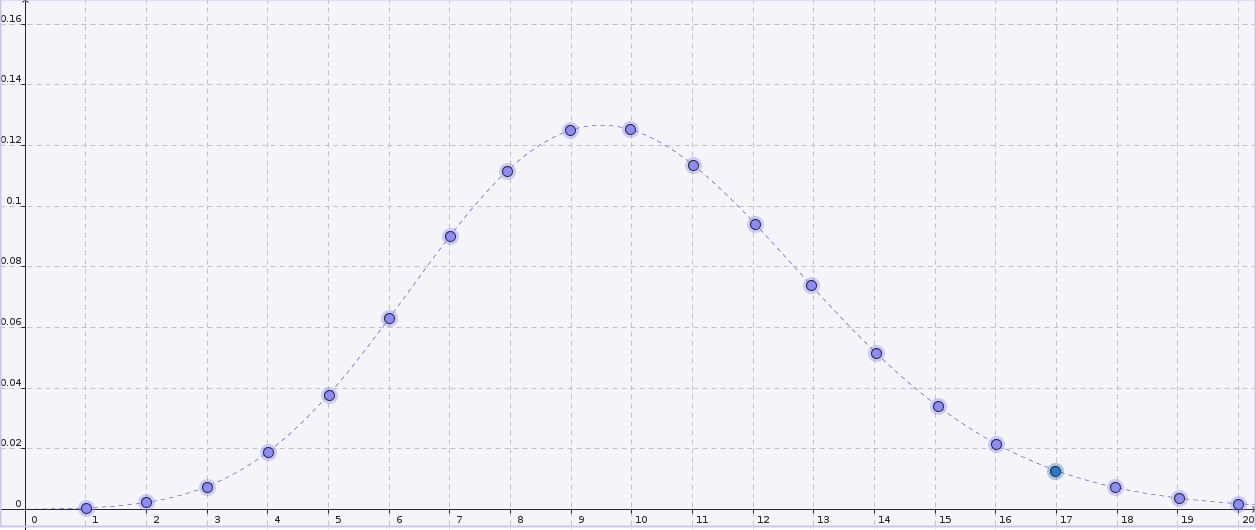
\includegraphics[width=15cm]{Cap1-Probabilidad/img/poisson.png}
        \caption{Gráfica de la probabilidad de que en determinado tiempo haya 'x' bacterias $cm^2$ de cultivo cuando la tasa media es $10$.}
    \end{figure}
\end{Ejm}
Esta distribución es una de las más importantes de una variable discreta. Sus principales aplicaciones hacen referencia a la modelización de situaciones en las que nos interesa determinar el número de hechos de cierto tipo que se pueden producir en un intervalo de tiempo o de espacio, bajo presupuestos de aleatoriedad y ciertas circunstancias restrictivas.\\
Esta distribución se puede hacer derivar de un proceso experimental de observación en el que tengamos las siguientes características.
\begin{itemize}
    \item El experimento debe ser aleatorio.
    \item Se observa el experimento durante un cierto periodo de tiempo o a lo largo de un espacio de observación.
    \item La probabilidad de que se produzcan un número $n$ de éxitos en un intervalo de amplitud $t$ no depende del origen del intervalo (aunque, sí de su amplitud).
    \item La probabilidad de que ocurra un hecho en un intervalo infinitésimo es prácticamente proporcional a la amplitud del intervalo.
    \item La probabilidad de que se produzcan $2$ o más hechos en un intervalo infinitésimo es un infinitésimo de orden superior a dos.
\end{itemize}
Gracias a estas características podemos identificar cuando nos encontramos en el caso de una distribución de Poisson. \\\\
%%%%%%%%%%%%%%%%%%%%%% DISTRIBUCIÓN BINOMIAL %%%%%%%%%%%%%%%%%%%%%
Otra distribución sumamente útil es la binomial, para cual primera será necesario definir la distribución de Bernoulli.\\ Esta distribución se define como aquel experimento aleatorio con únicamente dos posibles resultados, llamados genéricamente: éxito y fracaso.
Supondremos que las probabilidades de estos resultados son $p$ y $1-p$, respectivamente. Si se define la variable aleatoria $X$ como aquella función que lleva el resultado éxito al número $1$ y el resultado fracaso al número $0$, entonces decimos que $X$ tiene una distribución Bernoulli con parámetro $p\in[0,1]$.\\
Ahora, supongamos que efectuamos una serie de $n$  ensayos independientes Bernoulli en donde la probabilidad de éxito en cada ensayo es $p$. Si denotamos por $E$ el resultado éxito y por $F$ el resultado fracaso, entonces el espacio muestral de este experimento consiste de todas las posibles sucesiones de longitud $n$ de caracteres $E$ y $F$ . Así el espacio muestral consiste de $2^n$ elementos. Si ahora definimos la variable aleatoria $X$ como aquella función que indica el número de éxitos en cada una de estas sucesiones, esto es,
\begin{eqnarray*}
    X(E E\ldots E)=n\\ X(FE\ldots E)=n-1\\ \vdots\\X(F F\ldots F)=0
\end{eqnarray*}
Notamos que $X$  puede tomar los valores $0,1,\ldots,n$  y esta variable aleatoria devolverá el número de éxitos al realizar un número determinado de experimentos. Analicemos esto con un ejemplo.
\begin{Ejm}
    Se realiza un experimento con un tipo de fertilizante orgánico para eliminar el musgo en una plantación. Se encontró una efectividad en los primeros experimentos del $75\%$.
    Si se aplica el mismo fertilizante en $3$ parcelas del mismo tamaño y bajo las mismas condiciones, esto nos dice que tenemos $3$ ensayos independientes Bernoulli con probabilidad de éxito de $p=0.75$  cada una.\\
    Nuestro espacio muestral estaría conformado por $$\Omega= \{E E E,\thinspace F E E,\thinspace E F E,\thinspace E E F,\thinspace F F E,\thinspace F E F,\thinspace E F F,\thinspace F F F\}$$
    La probabilidad de obtener que $2$ parcelas no pierdan su cosecha es preliminarmente,
    \begin{eqnarray}
        \label{eq-ejm-binomial-fertilizante}
    	p\thinspace p (1-p)=(0.75)^2(0.25)
    \end{eqnarray}
    Aquí hemos colocado los $2$ éxitos en los primeros ensayos, cuando ello no ocurrirá necesariamente así. Las diferentes formas en que los $2$ éxitos pueden distribuirse de $3$ formas distintas $(F E E,\thinspace E F E,\thinspace E E F)$, al multiplicarlo con (\ref{eq-ejm-binomial-fertilizante}) obtenemos la probabilidad que deseamos. $$3(0.75)^2(0.25)$$
\end{Ejm}

En general, las diferentes formas en que los $x$ éxitos pueden distribuirse en los $n$ ensayos está dada por el coeficiente binomial $n\choose x$, al hacer la multiplicación de este coeficiente binomial con el término $p^x(1-p)^{n-x}$ se obtiene la expresión de la función de probabilidad para esta distribución.
\begin{Def}
    Una variable aleatoria $X$ tiene una distribución binomial con parámetros $n$ y $p$ y se denota por $X\sim bin(n,p)$ si tiene por función de probabilidad
    $$f(x)=
    \begin{cases}
        {n \choose x} p^x(1-p)^{n-x}& x=0,1,\ldots,n\\0 & \textit{en otro caso}
    \end{cases}$$
\end{Def}
Un experimento se puede modelar con una distribución binomial si cumple que:
\begin{itemize}
    \item Sólo hay dos posibles sucesos resultantes del experimento:
    (éxito y fracaso).
    \item Las probabilidades de cada suceso son las mismas en cualquier realización del experimento ( $p$ y $1-p$ , respectivamente).
    \item Toda realización del experimento es independiente del resto.
\end{itemize}
Gracias a estas características podemos identificar cuando un experimento modela una distribución binomial.\\\\
%%%%%%%%%%%%%%%% DISTRIBUCIÓN EXPONENCIAL%%%%%%%%%%%%%%%%%%%%%%%%%%%%%%
\begin{Def}
    Decimos que una variable aleatoria continua $X$ tiene distribución exponencial con parámetro $\lambda>0$, cuando su función de densidad es
    $$\begin{cases}
        \lambda e^{-\lambda x}, & \mbox{si $x>0$}\\
        0, & \mbox{en otro caso}
    \end{cases}
    $$
\end{Def}
Se trata pues de una variable aleatoria continua con conjunto de valores el intervalo $[0,\infty)$. Esta distribución se usa para modelar tiempos de espera para la ocurrencia de un cierto evento.\\
A pesar de la sencillez analítica de sus funciones de definición, la distribución exponencial tiene una gran utilidad práctica ya que podemos considerarla como un modelo adecuado para la distribución de probabilidad del tiempo de espera entre dos hechos que sigan un proceso de Poisson.\\
Tiene una gran utilidad en los siguientes casos:
\begin{itemize}
    \item Distribución del tiempo de espera entre sucesos de un proceso de Poisson.
    \item Distribución del tiempo que transcurre hasta que se produce un fallo, si se cumple la condición que la probabilidad de producirse un fallo en un instante no depende del tiempo transcurrido.
\end{itemize}
%%%%%%%%%%%%%%%%%%%%
Existen muchas más distribuciones recurrentes para variables aleatorias discretas, pero las mencionadas serán de nuestro principal interés.
    \section{Esperanza y funciones generadoras}
Para lograr una mayor simplicidad, suele ser mejor describir las probabilidades con algunos valores típicos. Entre aquellos valores, la media o esperanza es la más importante. Su definición va de acuerdo con el concepto común de promedio. \\Las demostraciones de los resultados expuestos en este capítulo se pueden encontrar en
\\\\
Si en una población determinada, $30$ familias tienen $1$ hijo, $10$ familias tienen $2$ hijos , $7$ tienen $3$ hijos y $3$ tienen $4$ hijos. El número total de familias es $50=30+10+7+3$ y el número total de hijos es $83=1(30)+2(10)+3(7)+4(3)$\\
El número promedio de hijos por familia es 
\begin{eqnarray}
    \label{ejm-esperanza-inicio}
    \frac{83}{50}= 1\big(\frac{30}{50}\big)+2\big(\frac{10}{50}\big)+3\big(\frac{7}{50}\big)+4\big(\frac{3}{50}\big)
\end{eqnarray}
Si definimos nuestra variable aleatoria $X=$ \textit{"números de hijos por familia"} y $f$ la función de probabilidad asociada a $X$. Por la definición de probabilidad clásica se obtiene que $f(1)=\frac{30}{50}$, $f(2)=\frac{10}{50}$, $f(3)=\frac{7}{50}$, $f(4)=\frac{3}{50}$ que coincide con los valores expuestos en \ref{ejm-esperanza-inicio} los cuales al reemplazarlos obtenemos que el promedio de hijos por familia es $1f(1)+2f(2)+3f(3)+4f(4)$.\\Una generalización de esta situación induce a la siguiente definición.
\begin{Def}
    Sea $X$ una variable aleatoria discreta que toma los valores $x_1,x_2,x_3,\ldots$ con probabilidades $f(x_1), f(x_2),\ldots$, la esperanza se define por $$E(X)=\sum x_k f(x_k)$$. Con la condición de que la serie converja absolutamente. En este caso decimos que $X$ tiene esperanza finita.
\end{Def}
Intuitivamente, la esperanza de una variable aleatoria $X$ representa la cantidad promedio que se "espera" como resultado de un experimento aleatorio cuando la probabilidad de cada suceso se mantiene constante y el experimento se repite un elevado número de veces. Cabe decir que el valor que toma la esperanza matemática en algunos casos puede no ser "esperado" en el sentido más general de la palabra (el valor de la esperanza puede ser improbable o incluso imposible). 
\begin{Ejm}
    El cálculo del valor esperado de la variable aleatoria nuestro ejemplo \ref{ejm-variableAleatoria-carros} estaría dado por
    \begin{eqnarray}
       E(X)= 0\frac{20}{30}+1\frac{6}{30}+2\frac{6}{30}+3\frac{3}{30}=\frac{1}{2}
    \end{eqnarray}
    La multiplicación de cada valor de $x$ por su probabilidad $f(x)$ proporciona los $xf(x)$ valores en la tercera columna. Siguiendo la definición de esperanza, sumamos esta columna,a $x f(x)$, para obtener la esperanza de $\frac{1}{2}$ automóviles vendidos por día. Cabe destacar que $0,5$ no es un valor posible.
\end{Ejm}
\begin{Def}
    \label{def-prob-funcionGeneraProb}
    Consideremos una variable aleatoria discreta $X$, que toma valores en el conjunto de estados $S=\{x_1,x_2,\ldots\}$ con distribución de probabilidad $\{p_k\}_{k\in\N}$, tal que $$p_k=P(X=x_k)$$ 
    La función generadora de probabilidad ($f.g.p.$) $G$ asociada a la variable aleatoria $X$ (o equivalentemente a su distribución $\{p_k\}$) es una función que se define por 
    \begin{eqnarray}
        G_X(s)=E(s^X)=\sum_{k=0}^\infty p_k s^{x_k} \label{def-funcionGeneradoraProb}
    \end{eqnarray} 
    donde,  $|s|\leq 1$.
\end{Def}
Como $\{f(x_k)\thinspace|\thinspace x_k\in S\}$ es una distribución de probabilidad, entonces\\ $\sum_{k=0}^\infty p_k=1$, por lo tanto, la serie definida en (\ref{def-funcionGeneradoraProb}) converge absolutamente para $|s|\leq 1$ pues $$|G(s)|\leq \sum_{k=0}^\infty|s|^k p_k\leq\suma p_k=1 $$ 
Como su nombre lo menciona, la $f.g.p.$ genera la probabilidad asociada a su distribución.
Notamos que al derivar la $f.g.p$ y evaluarlarlo en $0$ se obtiene que
$$G(0)=p_0$$ $$G'(0)=p_1$$ $$G''(0)=2!P_2$$ $$\vdots$$Desde que la serie (\ref{def-funcionGeneradoraProb}) converge absolutamente cuando $|s|\leq 1$, entonces es infinitamente diferenciable en el intervalo de convergencia. En general, por inducción se demuestra que la $k-$ésima derivada de la $f.g.p.$ de $X$ es $$G^{(k)}(0)=k!p_k$$
De esta forma obtenemos que $$p_k=\frac{G^{(k)}(0)}{k!}$$ recuperando lo que inicialmente era nuestra distribución de probabilidad.\\\\
\begin{Ejm}
    Supongamos que un experimento consiste en lanzar una moneda. Los posibles resultados son cara $C$ o sello $S$. Si $X$ es una variable aleatoria tal que $X(C)=1$, $X(S)=0$ con $P(X=0)=\frac{3}{4}$ y $P(X=1)=\frac{1}{4}$
    Por lo tanto la función generadora de probabilidad es
    $$G(s)=\frac{3}{4}+\frac{s}{4}.$$
    Ahora supongamos que no sabemos la distribución de probabilidad al lanzar esta moneda , pero sí se sabe que la función generadora de probabilidad asociada que es $G(s)=\frac{3}{4}+\frac{s}{4}.$\\
    Se verifica la reconstrucción de la función de probabilidad
    $$P(X=0)=G(0)=\frac{3}{4}.$$    $$P(X=1)=G'(0)=\frac{1}{4}.$$
\end{Ejm}
La función generadora de probabilidad determina de manera única a la distribución en el siguiente sentido. Si $X$ y $Y$ tienen la misma distribución de probabilidad, entonces naturalmente $E(X)=E(Y)$ lo cual implica también que $G_X=G_Y$, para valores donde esta esperanza exista.\\
Inversamente, sean $X$ y $Y$ tales que $G_X$ y
$G_Y$ existen y coinciden en algún intervalo no trivial alrededor del cero,
entonces $X$ y $Y$ tienen la misma distribución. Estas y otras propiedades
generales de la $f.g.p.$ se estudian a continuación.
\begin{Prop}
    Sean $X$ e $Y$ variables aleatorias con valores enteros no negativos tales que $G_X(s)$ y $G_Y(s)$ coinciden en algún intervalo alrededor de $s=0$. Entonces $X$ y $Y$ tienen la misma distribución de probabilidad. \label{prop-funcionGenIgual-distribucuionIgual}
\end{Prop}
\begin{Prop}
    Sean $X$  $Y$ independientes con f.g.p. $G_X$ y $G_Y$ respectivamente, entonces $G_{X+Y}(s)=G_X(s)G_Y(s)$
    \label{prop-funcionGenSuma-productoFuncionGen}
\end{Prop}
\begin{Def} 
    La función de probabilidad de dos valores aleatorios $X, Y$ con valores reales discretos en $\N$ es la función $f_{X,Y} :\R^2 \rightarrow [0, 1]$ dada por
    $$f(x,y)=
    \begin{cases}
        P(X=x,\thinspace Y=y), & \mbox{$x,y=1,2,\ldots$}\\
        0,& \mbox{en otro caso}
    \end{cases}$$
    A esta función se le llama función de probabilidad conjunta de las variables $X$ e $Y$.
\end{Def}
Sean $X$ y $Y$ variables aleatorias independientes, con valores enteros no negativos y con distribuciones de probabilidad $\{a_j\}_{j\in\N}$ y $\{b_k\}_{k\in\N}$ respectivamente, donde $a_j=P(X=j)$ y  $b_k=P(Y=k)$ $j,k\in\N$ , entonces $P(X=j,Y=k)=a_j b_k$.\\ La suma $X+Y$ es una nueva variable aleatoria por la proposición (\ref{prop-variableAl-X+YesVA}), y se cumple que $$(X+Y=m)=\bigcup_{j=0}^{m}(X=j,Y=m-j)$$ \\ Por lo tanto la distribución de la variable aleatoria $X+Y$, $\{c_m\}_{m\in\N}$, donde $c_m=P(X+Y=m)$, viene dada por
\begin{eqnarray}
    c_m=\sum_{j=0}^m P(X=j,Y=m-j)=\sum_{j=0}^m a_j b_{m-j}\label{def-convolucion}
\end{eqnarray}
La nueva distribución de probabilidad \ref{def-convolucion} que parte de las dos sucesiones $\{a_k\}$ y $\{b_k\}$ y conduce a una nueva sucesión $\{c_k\}$ ocurre con tanta frecuencia que es conveniente darle un nombre y una notación especial para ella
\begin{Def}
    Sean $\{a_k\}$ y $\{b_k\}$ dos sucesiones de enteros no negativos (no necesariamente distribuciones de probabilidades). La nueva sucesión $\{c_m\}$ definida en \ref{def-convolucion}, se llamará convolución de $a_k$ y $b_k$, y se denotará por
    \begin{eqnarray}
        \{c_k\}=\{a_k\}*\{b_k\}
        \label{def-notaciónConvolucion}
    \end{eqnarray}
\end{Def}
\begin{Obs}
    Si $f_X(k)=\{a_k\}$ y $f_Y(k)=\{b_k\}$ son funciones de probabilidad de las variables aleatorias $X$ e $Y$ respectivamente, denotaremos a la convolución $c_k=(f_X*f_Y)(k)$
\end{Obs}
\begin{Ejm}
    Si $a_k=b_k=1$ para toda $k=0,1,2,\ldots$, entonces $c_k=\sum_{j=0}^k 1=k+1$.\\Si $a_k=k$ y $b_k=1$, entonces $c_k=\sum_{j=0}^k j =\frac{k+k+1}{2}$.\\Finalmente, si $a_0=a_1=\frac{1}{2}$ y $a_k=0$ para $k\geq 2$ entonces $c_k=\frac{b_k+b_k-1}{2} $ 
\end{Ejm}

\chapter{Cocientes demográficos}
    %https://apuntesdedemografia.com/curso-de-demografia/cocientes-demograficos-tasas-probabilidades-razones-y-proporciones/%
    %https://thales.cica.es/rd/Recursos/rd98/Medicina/01/p_stock.html%
    El puro dato normalmente es poco útil. 5000 nacimientos no nos dicen nada si no sabemos en qué población se han producido. Y, aún peor, las series larguísimas de datos tampoco son casi nunca útiles, porque resultan casi imposibles de entender o interpretar. Por eso en demografía se trabaja con “indicadores” en los que se relacionan o resumen otros datos.
    %\section{Tipos de cocientes más relevantes}
En análisis demográfico existen cuatro tipos de tales divisiones o cocientes, distinguidos en función del tipo de datos que constituyen respectivamente el numerador y el denominador.
\begin{itemize}
    \item Cuando ambos números son el mismo tipo de magnitud, bien flujos, bien stocks.
    \begin{enumerate}
        \item Proporción. Cociente que resulta de dividir un subconjunto por el conjunto total en el que está incluido.\\
        Por ejemplo, las mujeres de una población respecto a la población total.
        \item Razón. Cociente que resulta de dividir dos conjuntos o subconjuntos distintos que no tienen elementos comunes. Por ejemplo, los hombres de una población respecto a las mujeres de esa misma población, la llamada "razón de masculinidad".
    \end{enumerate}
    \item Cuando el numerador es un flujo de acontecimientos y sólo el denominador es un stock poblacional.
    \begin{enumerate}
        \item Tasa. Cociente que resulta de dividir un número de acontecimientos sucedidos durante un periodo de tiempo (un flujo) por la población media existente durante ese periodo.\\Por ejemplo la tasa de mortalidad es el número de defunciones durante un periodo de tiempo, dividido por la población media de ese mismo periodo. \\ Lo que diferencia las tasas de las proporciones es que en el numerador se sitúan flujos, es decir, acontecimientos registrados durante cierto periodo, mientras que el denominador corresponde a un stock y, por tanto, se refiere a un instante.
        \item Probabilidad. Cociente entre los acontecimientos experimentados por una población durante un periodo de tiempo y la población inicial de dicho periodo, susceptible de experimentar tales acontecimientos.Adoptan la forma de una fracción en que la población afectada ocupa el numerador y en el denominador (abajo) se sitúa la población que podría en principio haber estado afectada.\\Por ejemplo, la probabilidad de morir entre los 20 y los 22 años para la generación 1970 se calcula dividiendo las defunciones de miembros de esta generación, en ese intervalo de edades, por el número de sus integrantes que se encontraban con vida al cumplir los 20 años exactos.
    \end{enumerate}
\end{itemize}
El análisis demográfico permiten mejorar la toma de decisiones y hacer pronósticos sobre determinadas cuestiones, por ejemplo, en torno a la salud, a determinadas acciones a tomar frente un catástrofe o a las políticas económicas.

    \section{Ideas preliminares}
Considere un experimento aleatorio y suponga que evoluciona o cambia de un estado a otro a lo largo del tiempo y sea $X_t$ el estado del experimento al tiempo $t$, de tal forma que cada $X_t$ es una variable aleatoria para cada $t$. Esta colección de variables aleatorias se conoce como proceso estocástico, y sirve como modelo para representar la evolución aleatoria de un sistema a lo largo del tiempo.\\
Las demostraciones de los resultados expuestos en este capítulo se pueden encontrar en \cite{Feller}, \cite{Rincon3} \\
\begin{Def}
    Un proceso estocástico de define como una colección de variables aleatorias $\{X_t\}_{t\in T}$ definidas en algún espacio de probabilidad $(\Omega,\thinspace\mathscr{F})$, que es parametrizada por un conjunto $T$ ( el cual es llamado espacio parametral), en donde las variables aleatorias toman valores en un conjunto $S$ denominado espacio de estados.
\end{Def}
Un proceso estocástico puede interpretarse como una sucesión de variables aleatorias cuyas características pueden variar a lo largo del tiempo.
Puede tenerse un espacio de estado discreto o un espacio de estado continuo. En el caso más simple, se utiliza un conjunto discreto como espacio de parámetros $T= \{0, 1, 2,\ldots\}$ y estos números se interpretan como tiempos épocas. En este caso se dice que el proceso es a tiempo discreto (también conocido como cadenas), este tipo
de procesos será denotado en general por $\{X_n\}^{\infty}_{n=0}$, o $\{X_n:\thinspace n= 0, 1, \ldots\}$ dependiendo de la complejidad de la notación de la variable aleatoria a utilizar.\\Por lo tanto para cada $n$, se tiene que $X_n$ vendría a ser el valor del proceso o estado del sistema al tiempo $n$.
Se puede tomar como ejemplo a los cambios que podrían ocurrir "cada día, cada mes, cada año, etc."\\ En el caso del tiempo continuo, el espacio parametral se considera como el conjunto continuo $T=[0,+\infty)$ donde los cambios de estado se podrían realizar en cualquier instante.\\
A partir de ahora, seguiremos la convención de si el subíndice de la variable aleatoria es denotada con $n$, entonces el espacio parametral será discreta, mientras que si el subíndice es $t$, el tiempo se medirá de manera continua.\\
\begin{Ejm}
    Considere una máquina en una fábrica. Un posible estado de la máquina es si está funcionando o no, esta verificación se realiza al comienzo de cada día hábil. Se le asigna el estado "inactivo" a un valor de $0$ y el estado "activo" a un valor de $1$. Una colección de variables aleatorias es proporcionada por.
    $$X_t=
    \label{ejm-procEstocástico}
    \begin{cases}
        0, & \mbox{Si la máquina está 'inactivo' en el tiempo $t$}\\
        1, & \mbox{Si la máquina está 'activo' en el tiempo $t$}
    \end{cases}$$
    La figura (\ref{fig-procesoEstocástico-Ejemplo}) muestra una posible secuencia de cambios de estado a través del tiempo para esa máquina.
    \begin{center}
        \begin{figure}[htb]
            \begin{center}
             \includegraphics[width=14cm]{Cap2-ProcesosEstocásticos/img/ejem1.JPG}
                \vspace*{0.05in}
            \end{center}
            \caption{Estado que se encuentra la máquina al tiempo $t$ }
            \label{fig-procesoEstocástico-Ejemplo}
        \end{figure}
    \end{center}
    Según la gráfica, la máquina al tiempo $0$ y $1$ se encuentra en operación, por eso:
    $$X_0=1$$
    $$X_1=1$$
    Al tiempo $2$ la máquina cambia de estado y se encuentra fuera de funcionamiento. 
    $$X_2=0$$
   Sucesivamente vemos como la máquina va cambiando de estado constantemente a través del tiempo.
    $$X_3=1$$
    $$X_4=0$$
    $$\vdots$$
\end{Ejm}
\begin{Obs}
Para cualquier $t\in T$ se denota $P(X(t)=i)$, $P_t=i$ o $P(X_t=i)$ como la probabilidad que en el tiempo $t$ el ensayo está en el estado $i$, es decir $P(\omega\in\Omega,\thinspace X_t(\omega)=i).$
\end{Obs}
Un proceso estocástico, también llamado proceso aleatorio, puede considerarse como una función de dos variables
$$X:T\times\Omega\rightarrow S$$ a la cual a cada $(t,\thinspace\omega)$ se le asocia el valor o estado $X (t,\thinspace\omega) $.\\
Para cada valor aleatorio $t$ en $T$ , el mapeo $X_t$ , $X_t: \Omega\rightarrow S$ es una variable aleatoria, mientras que para cada $\omega$ en $\Omega$ fijo arbitrario, la función $X(\cdot\thinspace,\thinspace\omega)$ es llamada una trayectoria.\\En este trabajo estaremos interesados en el caso de procesos estocásticos con espacio de estados discreto, suele representarse de la siguiente
manera: $$(X_0=k_0,\thinspace\ldots,\thinspace X_n=k_n)$$
La principal preocupación de los estudios realizados en casos discretos es calcular la probabilidad de ocupación de cada estado a partir de la probabilidad particular de cambio de estado. ¿Con qué probabilidad se estará en el estado $k_n$ en el instante $n$ dado que en el instante $n-1$ el proceso se encontraba en el estado $k_{n-1}$? Esta probabilidad de denotará como:
$$P(X_n = k_n\mid X_{n-1} = k_{n-1})$$
A este tipo de probabilidad condicionada se le denomina probabilidad de transición o de cambio de estado. $P(X_n = k_n\mid X_{n-1} = k_{n-1})$. \\Otra forma de denotarlo es $P(X_n = k_n \mid X_{n-1} := k_{n-1})=P_{i j}{(n-1,n)}$
\begin{Ejm}
    Del proceso estocástico expuesto en el ejemplo (\ref{ejm-procEstocástico}), \\$P_{0,1}(n-1,n)=P(X_n=1\mid X_{n-1}=0)$ denota la probabilidad de que en el tiempo $n$ la máquina esté 'en operación' , dado que previamente en el tiempo $n-1$ se encontraría 'fuera de funcionamiento'.\\
    $P_{1,0}(n-1,n)=P(X_{n-1}=0\mid X_n=1)$ denota la probabilidad de que en el tiempo $n$ la máquina se encuentre 'fuera de funcionamiento', dado que previamente en el tiempo $n-1$ estaba 'en operación'.\\
    $P_{0,0}(n-1,n)=P(X_{n-1}=0\mid X_n=0)$ denota la probabilidad de que en el tiempo $n$ la máquina esté 'fuera de funcionamiento', dado que previamente en el tiempo $n-1$ también se encontraba 'fuera de funcionamiento'.
\end{Ejm}
Una propiedad interesante que se presentan en algunas cadenas es que los valores de sus probabilidades de transición no dependan del valor de $n$. Es decir, "las probabilidades de cambiar de estado son las mismas en cualquier instante y no dependen del tiempo en que se encuentre el experimento, más bien lo relevante es el tiempo que transcurre durante la transición de estados". Esto es $$P_{i j}(0,n)=P_{i,j}(k,k+n),\quad \forall k\in\N$$.\\
A este tipo de transiciones se le conoce como estacionarias y se denotan por simplicidad $P_{i,j}(n)$, en vez de $P_{i,j}(k,k+n)$ para cualquier $k\in T$, de esta manera se resalta que el tiempo transcurrido es $n$.\\
\begin{Obs}
    Sea $P_{i,j}(m,n)$ una probabilidad de transición estacionaria arbitraria. Por definición tenemos que $P_{i,j}(m,n)=P_{i,j}(n-m)$
\end{Obs}
\begin{Def}
    Sea  $\{X_t\}_{t\in T}$ un proceso estocástico con valores en el conjunto de estados $S=\{x_0,\thinspace x_1,\thinspace x_2 ,\ldots\}$ ( S puede ser finito o numerable ).
    Decimos que $\{X_t\}_{t\in T}$ es una cadena de Markov si cumple la siguiente propiedad conocida como la condición de Markov
    \begin{eqnarray}
    P(X_{n+1}=k_{n+1}\mid  X_{0}=k_0,\thinspace\ldots,\thinspace X_{n}=k_n)=P(X_{n+1}=k_{n+1}\mid X_{n}=k_n)
    \label{procesosEstocásticos-condMarkov}
    \end{eqnarray}
    Esto significa que la probabilidad de que el suceso $k_{n+1}$ ocurra en el tiempo $n+1$ (futuro) solo dependerá de la ocurrencia del evento $k_n$ en el tiempo $n$ (presente), mientras que la información de lo que ocurrió en los tiempos $0,\thinspace 1,\thinspace 2, \ldots,n-1$ (pasado) es irrelevante.
\end{Def}
\begin{Teo}
    La condición de Markov (\ref{procesosEstocásticos-condMarkov}) es equivalente a poder calcular la distribución conjunta de las variables $\{X_k\}_{k=1}^n$ de la siguiente forma:
    \begin{eqnarray}
    \label{procesosEstocásticos-condMarkovEquiv}
    P(X_0= k_0,\thinspace\ldots,X_{n+1}= k_{n+1}) =P(X_0=k_0)P(X_1=k_1|\thinspace X_0=k_0)\cdots P(X_{n+1}=k_{n+1}|\thinspace X_n=k_n)
    \end{eqnarray}
\end{Teo}
Puede considerarse que la denominada cadena de Markov inicia su evolución iniciando en un estado $i$ cualquiera, o de manera más generalizada considerando una
distribución de probabilidad inicial sobre un espacio de estados. Una distribución inicial para una cadena de Markov con espacio de estados $t= 0, 1,\thinspace 2,\thinspace,\ldots  $ es simplemente una distribución de probabilidad sobre este conjunto, es decir,
es un conjunto de números $p_0,\thinspace p_1,\thinspace p_2 ,\ldots >0$ cuya suma converge a uno. El número $p_i$ corresponde a la probabilidad de que la cadena inicie en el estado $i$, es decir $P(X_0= i)$\\ \\
\begin{Obs}
    En las cadenas de Markov en tiempo discreto, utilizamos como índice un tiempo
    discreto $n=0, 1, 2,\ldots$ y se deducían numerosas propiedades.
    Las nociones de cadenas de Markov se puede extender a un tiempo continuo $t \geq 0$.
\end{Obs}
Consideremos un proceso a tiempo continuo $\{X_t\}_{t\geq 0}$ que inicia en un estado $i_1$.
\begin{figure}
    \centering
    \includegraphics[width=10cm]{Cap2-ProcesosEstocásticos/img/procesos_continuos.png}
    \caption{Proceso estocástico a tiempo continuo}
    \label{fig-procEstocastContinuo}
\end{figure}
El proceso permanece en ese estado un tiempo $T_{i 1}$ y
después toma el valor de un nuevo estado $i_2$ distinto del anterior, permanece en ese estado un tiempo determinado $T_{i 2}$ hasta llegar a un estado posterior y así sucesivamente. Esta
sucesión de saltos se muestra gráficamente en la figura \ref{fig-procEstocastContinuo}
Los tiempos aleatorios $T_{i_j}$ son aquellos
en los que el proceso permanece constante en alguno de sus estados, son denominados tiempos de estancia.
Los momentos en donde el proceso cuenta con "saltos" son los tiempos $W_n=T_{i_1}+\cdots+T_{i_n}$ $n\in\N$.
Nuestro proceso estocástico $\{X_t\}_{t\geq 0}$ puede ser descrito como:
 $$X_t =
 \begin{cases}
    i_1, & \mbox{ Si $0\leq t <W_1$}\\
    i_2, & \mbox{ Si $0\leq t <W_2$}\\
    i_3, & \mbox{ Si $0\leq t <W_3$}\\
    \vdots
 \end{cases}$$
\begin{Def}
    Sea $\{X_t\}_{t\geq 0}$ un proceso estocástico sobre el conjunto de estados $S$, es una cadena de Markov de tiempo continuo si $S$ es numerable y para cualquier $0\leq t_1<t_2<\ldots<t_n<t_{n+1}$ se tiene  $$P\big(X_{t_n}=i_n\mid X_{t_1}=i_{t_1},\ldots ,\thinspace X_{t_{n-1}}=i_{t_{n-1}}\thinspace \big)=P\big(X_{t_n}=i_n\mid X_{t_{n-1}}=i_{t_{n-1}}\big)$$
\end{Def}
Observe que no estamos suponiendo el conocimiento de la historia previa del suceso, si no, únicamente en una colección finita arbitraria de tiempos pasados $t_1,t_2,t_3,\ldots,t_{n-1}$.\\
Supondremos nuevamente que estas probabilidades de transición son estacionarias en el tiempo (para cada $s\leq 0$ y $t\leq 0$, la probabilidad $P(X_{t+s} =j \mid X_s= i)$ 
es idéntica a $P(X _{t} =j \mid X_0= i)$), esta probabilidad se denota mediante la expresión $P_{i j}(t)$, para $i$ y $j$ enteros no negativos.\\
\begin{Obs}
    En particular para $t= 0$, tanto para el caso continuo como discreto, se define la probabilidad de transición $P_{i j}(0)$ como la función delta de Kronecker, es decir,
    $$P_{i,j}(0)=\delta_{i j}=\begin{cases}
        1, & \mbox{Si $i=j$}\\
        0, & \mbox{Si $i\not= j$}
    \end{cases}$$
    Esto nos da a entender que, cuando el tiempo aún no transcurre ( se encuentra en la etapa inicial ), la probabilidad de que ocurra un cambio es nula, mientras que la probabilidad de que permanezca en el mismo estado ( que no cambie ) es absoluta, es decir $1$.
\end{Obs}
Cuando los índices $i$ y $j$ varían, por ejemplo, sobre el conjunto de estados $t=\{ 1,\thinspace 2,\ldots, n\}$ , se le conoce como matriz de probabilidades de transición de paso $t$, $t\geq 0$
$$P(t)=\left( \begin{array}{ccc}
p_{0 0}(t) & \cdots & p_{0 n}(t) \\ 
p_{1 0}(t) & \cdots & p_{1 n}(t)\\
\vdots & \ddots & \vdots \\
p_{n 0}(t) & \cdots & p_{n n}(t) 
\end{array}\right)\\$$
\begin{Ejm}
    En Perú existen $3$ operadores principales de telefonía móvil como lo son Movistar, Claro y Entel (estados).
    Los porcentajes actuales que tiene cada operador en el mercado actual son para Movistar $0.4$ para Claro $0.25$ y para Entel $0.35$. (estado inicial).
    Un usuario de Movistar actual tiene una probabilidad de permanecer en Movistar de $0.60$, una probabilidad de cambiar a Claro de $0.2$ y la probabilidad de pasarse a Entel de $0.2$.\\Por otro lado, si el usuario es cliente de Claro tiene una probabilidad de mantenerse en Claro del $0.5$, de que esta persona se cambie a Movistar  $0.3$ y que se pase a Entel de $0.2$.\\Y si el usuario es cliente de Entel la probabilidad que permanezca es de $0.4$, de que se cambie a Movistar de $0.3$ y a Claro de $0.3$.\\
    Nuestra proceso estocástico estaría dado por $\{X_t\}_{t\leq 0}$ donde para dado tiempo $t\geq 0$, $\thinspace X_t(Movistar)=0$ ,$\thinspace X_t(Claro)=1$, $\thinspace X_t(Entel)=2$, partiendo de esta información podemos elaborar la matriz de transición.
   $$P(1)=\left( \begin{array}{ccc}
    P_{0 0}(1) & P_{0 1}(1) & P_{0 2}(1) \\
    P_{1 0}(1) & P_{1 1}(1) & P_{1 2}(1) \\
    P_{2 0}(1) & P_{2 1}(1) & P_{2 2}(1)  
    \end{array}\right)=
    \left( \begin{array}{ccc}
    0.60 & 0.2 & 0.2 \\ 
    0.3 & 0.5 & 0.2 \\
    0.3 & 0.3 & 0.4
    \end{array}\right)\\$$
    La suma de las probabilidades de cada estado (en este caso el operador telefónico) deben ser iguales a $1$. Nuestro estado inicial en este caso sería $$P(X_0 = 0)= 0.4,\thinspace P(X_0 = 1)= 0.25 ,\thinspace P(X_0 = 2)= 0.35$$
    Para descubrir el valor de la probabilidad de una persona usando Movistar en la época $0$ y luego empiece a usar Claro en la época $1$. 
    $$P(X_1=1 , X_0=0) = P(X_0=0)P_{01}(1)= 0.40\cdot 0.20 =0.08$$
    Para descubrir el valor de la probabilidad de que una persona use Entel en la época $0$ y luego empiece a usar Movistar en la época $1$ está dado por
    $$P(X_1=0 , X_0=2) = P(X_0=2)P_{20}(1)=0.35\cdot 0.3 =0.105$$
    y si suponemos que nuestro proceso estocástico cumple la condición de Markov (\ref{procesosEstocásticos-condMarkov}) de pérdida de memoria, (no nos importa qu\'e operador us\'o  mucho antes, solo nos interesa el operador usado previamente antes de la transición) entonces para calcular, por ejemplo la probabilidad de que una persona use Movistar en la época $0$, luego use Claro en la época $1$ y finalmente Entel en la época $2$ usamos la condición equivalente (\ref{procesosEstocásticos-condMarkovEquiv}).
    $$P(X_2=2,\thinspace X_1=1,\thinspace X_0=0)=P(X_0=0)P_{01}(1)P_{12}(1)=0.4\cdot 0.2\cdot 0.2=0.016$$
    \end{Ejm}
    De esta forma encontramos que la probabilidad de que una persona elija Movistar y luego se cambie de operador a Movistar y finalmente acabe usando Entel es $0.016$.
\begin{comment}
    \begin{Teo}(Ecuación de Chapman-Kolmogorov)
        Para cualquier
        par de números enteros $m$ y $n$ tales que $0\leq m\leq n$, y para cualesquiera estados $i$ y $j$ se cumple
        \begin{eqnarray}
            p_{i,j}(m,n)=\sum_k p_{i,k}(m,u)P(u,t)
        \end{eqnarray}
    \end{Teo}
\end{comment}
    \section{Tipos de cocientes más relevantes}
En análisis demográfico existen cuatro tipos de tales divisiones o cocientes, distinguidos en función del tipo de datos que constituyen respectivamente el numerador y el denominador.
\begin{itemize}
    \item Cuando ambos números son el mismo tipo de magnitud, bien flujos, bien stocks.
    \begin{enumerate}
        \item Proporción. Cociente que resulta de dividir un subconjunto por el conjunto total en el que está incluido.\\
        Por ejemplo, las mujeres de una población respecto a la población total.
        \item Razón. Cociente que resulta de dividir dos conjuntos o subconjuntos distintos que no tienen elementos comunes. Por ejemplo, los hombres de una población respecto a las mujeres de esa misma población, la llamada "razón de masculinidad".
    \end{enumerate}
    \item Cuando el numerador es un flujo de acontecimientos y sólo el denominador es un stock poblacional.
    \begin{enumerate}
        \item Tasa. Cociente que resulta de dividir un número de acontecimientos sucedidos durante un periodo de tiempo (un flujo) por la población media existente durante ese periodo.\\Por ejemplo la tasa de mortalidad es el número de defunciones durante un periodo de tiempo, dividido por la población media de ese mismo periodo. \\ Lo que diferencia las tasas de las proporciones es que en el numerador se sitúan flujos, es decir, acontecimientos registrados durante cierto periodo, mientras que el denominador corresponde a un stock y, por tanto, se refiere a un instante.
        \item Probabilidad. Cociente entre los acontecimientos experimentados por una población durante un periodo de tiempo y la población inicial de dicho periodo, susceptible de experimentar tales acontecimientos.Adoptan la forma de una fracción en que la población afectada ocupa el numerador y en el denominador (abajo) se sitúa la población que podría en principio haber estado afectada.\\Por ejemplo, la probabilidad de morir entre los 20 y los 22 años para la generación 1970 se calcula dividiendo las defunciones de miembros de esta generación, en ese intervalo de edades, por el número de sus integrantes que se encontraban con vida al cumplir los 20 años exactos.
    \end{enumerate}
\end{itemize}
El análisis demográfico permiten mejorar la toma de decisiones y hacer pronósticos sobre determinadas cuestiones, por ejemplo, en torno a la salud, a determinadas acciones a tomar frente un catástrofe o a las políticas económicas.

    %\section{Tipos de cocientes más relevantes}
En análisis demográfico existen cuatro tipos de tales divisiones o cocientes, distinguidos en función del tipo de datos que constituyen respectivamente el numerador y el denominador.
\begin{itemize}
    \item Cuando ambos números son el mismo tipo de magnitud, bien flujos, bien stocks.
    \begin{enumerate}
        \item Proporción. Cociente que resulta de dividir un subconjunto por el conjunto total en el que está incluido.\\
        Por ejemplo, las mujeres de una población respecto a la población total.
        \item Razón. Cociente que resulta de dividir dos conjuntos o subconjuntos distintos que no tienen elementos comunes. Por ejemplo, los hombres de una población respecto a las mujeres de esa misma población, la llamada "razón de masculinidad".
    \end{enumerate}
    \item Cuando el numerador es un flujo de acontecimientos y sólo el denominador es un stock poblacional.
    \begin{enumerate}
        \item Tasa. Cociente que resulta de dividir un número de acontecimientos sucedidos durante un periodo de tiempo (un flujo) por la población media existente durante ese periodo.\\Por ejemplo la tasa de mortalidad es el número de defunciones durante un periodo de tiempo, dividido por la población media de ese mismo periodo. \\ Lo que diferencia las tasas de las proporciones es que en el numerador se sitúan flujos, es decir, acontecimientos registrados durante cierto periodo, mientras que el denominador corresponde a un stock y, por tanto, se refiere a un instante.
        \item Probabilidad. Cociente entre los acontecimientos experimentados por una población durante un periodo de tiempo y la población inicial de dicho periodo, susceptible de experimentar tales acontecimientos.Adoptan la forma de una fracción en que la población afectada ocupa el numerador y en el denominador (abajo) se sitúa la población que podría en principio haber estado afectada.\\Por ejemplo, la probabilidad de morir entre los 20 y los 22 años para la generación 1970 se calcula dividiendo las defunciones de miembros de esta generación, en ese intervalo de edades, por el número de sus integrantes que se encontraban con vida al cumplir los 20 años exactos.
    \end{enumerate}
\end{itemize}
El análisis demográfico permiten mejorar la toma de decisiones y hacer pronósticos sobre determinadas cuestiones, por ejemplo, en torno a la salud, a determinadas acciones a tomar frente un catástrofe o a las políticas económicas.


\chapter{Procesos estocásticos que dependen del tiempo}
    En el estudio de las variables aleatorias realizado hasta ahora se han explorado las características aleatorias del fenómeno pero se ha mantenido una premisa por defecto, que esas
    características aleatorias permanecen constantes a través del tiempo. Al incluir en el estudio la presencia del tiempo se está considerando que de alguna forma la variable aleatoria depende del tiempo.
    En este capítulo estudiaremos procesos estocásticos en los que solo interviene una cantidad numerable de estados pero que dependen de un parámetro continuo del tiempo.
    \section{Ideas preliminares}
Considere un experimento aleatorio y suponga que evoluciona o cambia de un estado a otro a lo largo del tiempo, y sea $X_t$ el estado del experimento al tiempo $t$ de tal forma que puede considerarse
que $X_t$ es una variable aleatoria para cada valor del índice $t$. Esta colección de variables aleatorias es la definición de proceso estocástico, y sirve como modelo para representar la evolución aleatoria de un sistema a lo largo del tiempo.\\
Las demostraciones de los resultados expuestos en este capítulo se pueden encontrar en\\\\
\begin{Def}
    Un proceso estocástico es una colección de variables aleatorias $\{X_t\}_{t\in T}$ definidas en algún espacio de probabilidad $(\Omega,\thinspace\mathscr{F})$, parametrizada por un conjunto $T$, llamado espacio parametral, en donde las variables aleatorias toman valores en un conjunto $S$ llamado espacio de estados.
    Por tanto, un proceso estocástico puede interpretarse como una sucesión de variables aleatorias cuyas características pueden variar a lo largo del tiempo.
\end{Def}
Se puede tener un espacio de estados discreto y un espacio de estados continuo.
En los casos más sencillos se toma como espacio parametral el conjunto
discreto $T= \{0, 1, 2,\ldots\}$ y estos números se interpretan como tiempos. En este caso se dice que el proceso es a tiempo discreto (también conocido como cadenas), y en general este tipo
de procesos se denotará por $\{X_n:\thinspace n= 0, 1, \ldots\}$ , o $\{X_n:\thinspace n= 0, 1, \ldots\}$ dependiendo de la complejidad de la notación de la variable aleatoria a utilizar.\\Así, para cada $n$, $X_n$ es es el valor del proceso o estado del sistema al tiempo $n$.
Se podría tomar como ejemplo a los cambios de que ocurren cada día, cada mes, cada año, etc.\\ En el caso del tiempo continuo, el espacio parametral se considera como el conjunto continuo $T=[0,+\infty)$ donde los cambios de estado se podrían realizar en cualquier instante.\\
A partir de ahora, seguiremos la convención de que si el subíndice de la variable aleatoria es $n$, entonces los tiempos son discretos; y si el subíndice es $t$, el tiempo se mide de manera continua\\
\begin{Ejm}
    Considere una máquina dentro de una fábrica. Los
    posibles estados para la máquina son que esté operando o que esté fuera de funcionamiento
    y la verificación de esta característica se realizará al principio de cada día de trabajo. Si
    hacemos corresponder el estado 'fuera de funcionamiento' con el valor 0 y el estado 'en operación' con el valor 1, nuestra colección de variables aleatoria está dada por 
    $$X_t=
    \label{ejm-procEstocástico}
    \begin{cases}
        0, & \mbox{Si la máquina está 'fuera de funcionamiento' en el tiempo $t$}\\
        1, & \mbox{Si la máquina está 'en operación' en el tiempo $t$}
    \end{cases}$$
    La figura (\ref{fig-procesoEstocástico-Ejemplo}) muestra una posible secuencia de cambios de estado a través del tiempo para esa máquina.
    \begin{center}
        \begin{figure}[htb]
            \begin{center}
             \includegraphics[width=14cm]{Cap3-ProcesosEstocásticos/img/ejem1.JPG}
                \vspace*{0.05in}
            \end{center}
            \caption{Estado que se encuentra la máquina al tiempo $t$ }
            \label{fig-procesoEstocástico-Ejemplo}
        \end{figure}
    \end{center}
    Según la gráfica, la máquina al tiempo $0$ y $1$ se encuentra en operación, por eso:
    $$X_0=1$$
    $$X_1=1$$
    Al tiempo $2$ la máquina cambia de estado y se encuentra fuera de funcionamiento. 
    $$X_2=0$$
    Y así sucesivamente vemos como la máquina va cambiando de estado constantemente a través del tiempo.
    $$X_3=1$$
    $$X_4=0$$
    $$\vdots$$
\end{Ejm}
\begin{Obs}
Para cualquier $t\in T$ se denota $P(X_t=i)$ o $P(X_t=i)$ para representar a la probabilidad que en el tiempo $t$ el ensayo está en el estado $i$. Esto es  $P(\omega\in\Omega,\thinspace X_t(\omega)=i).$
\end{Obs}
Un proceso estocástico, también llamado proceso aleatorio, puede considerarse como una función de dos variables
$$X:T\times\Omega\rightarrow S$$ a la cual a cada $(t,\thinspace\omega)$ se le asocia el valor o estado $X (t,\thinspace\omega) $.\\
Para cada valor de $t$ en $T$ , el mapeo $X_t$ o $X_t$ es una variable aleatoria, mientras que para cada $\omega$ en $\Omega$ fijo, la función $X(\cdot\thinspace,\thinspace\omega)$ es llamada una trayectoria o realización del proceso.\\En este trabajo estaremos interesados en el caso de procesos estocásticos con espacio de estados discreto, suele representarse de la siguiente
manera: $$(X_0=k_0,\thinspace\ldots,\thinspace X_n=k_n)$$
El principal interés del estudio a realizar en el caso discreto es el cálculo de probabilidades de ocupación de cada estado a partir de las probabilidades de cambio de estado. Si en el instante $n-1$ se encontraba en el estado $k_{n-1}$, ¿Con qué probabilidad se estará en el estado $k_n$ en
el estado siguiente $n$? Esta probabilidad de denotará como:
$$P(X_n = k_n\thinspace | \thinspace X_{n-1} = k_{n-1})$$
A este tipo de probabilidad condicionada se le denomina probabilidad de transición o de cambio de estado.\\Otra forma de denotarlo es $P(X_n = k_n\thinspace | \thinspace X_{n-1} := k_{n-1})=P_{i j}{(n-1,n)}$
\begin{Ejm}
    Del proceso estocástico expuesto en el ejemplo (\ref{ejm-procEstocástico}), \\$P_{0,1}(n-1,n)=P(X_n=1\thinspace|\thinspace X_{n-1}=0)$ denota la probabilidad de que en el tiempo $n$ la máquina esté 'en operación' , si previamente en el tiempo $n-1$ estaba 'fuera de funcionamiento'.\\
    $P_{1,0}(n-1,n)=P(X_{n-1}=0\thinspace|\thinspace X_n=1)$ denota la probabilidad de que en el tiempo $n$ la máquina esté 'fuera de funcionamiento', si previamente en el tiempo $n-1$ estaba 'en operación'.\\
    $P_{0,0}(n-1,n)=P(X_{n-1}=0\thinspace|\thinspace X_n=0)$ denota la probabilidad de que en el tiempo $n$ la máquina esté 'fuera de funcionamiento', si previamente en el tiempo $n-1$ también se encontraba 'fuera de funcionamiento'.
\end{Ejm}
Una propiedad interesante que se presentan en algunas cadenas es que los valores de sus probabilidades de transición no dependan del valor de $n$. Es decir, las probabilidades de cambiar de estado son las mismas en cualquier instante y no dependen del tiempo en que se encuentre el experimento, más bien lo relevante es el tiempo que transcurre en la transición. Esto es $$P_{i j}(0,n)=P_{i,j}(k,k+n),\quad \forall k\in\N$$ Por simplicidad se asumirá tal situación.\\
A este tipo de transiciones se le conoce como estacionarias y se denotan por simplicidad $P_{i,j}(n)$, en vez de $P_{i,j}(k,k+n)$ para cualquier $k\in T$, de esta manera se resalta que el tiempo transcurrido es $n$.\\
\begin{Obs}
    Sea $P_{i,j}(m,n)$ una probabilidad de transición estacionaria arbitraria. Por definición tenemos que $P_{i,j}(m,n)=P_{i,j}(n-m)$
\end{Obs}
\begin{Def}
    Sea  $\{X_t\}_{t\in T}$ un proceso estocástico con valores en el conjunto de estados $S=\{x_0,\thinspace x_1,\thinspace x_2 ,\ldots\}$ ( S puede ser finito o numerable ).
    Decimos que $\{X_t\}_{t\in T}$ es una cadena de Markov si cumple la siguiente propiedad conocida como la condición de Markov
    \begin{eqnarray}
    P(X_{n+1}=k_{n+1}\thinspace|\thinspace  X_{0}=k_0,\thinspace\ldots,\thinspace X_{n}=k_n)=P(X_{n+1}=k_{n+1}\thinspace|\thinspace X_{n}=k_n)
    \label{procesosEstocásticos-condMarkov}
    \end{eqnarray}
    Esto significa que la probabilidad de que el suceso $k_{n+1}$ ocurra en el tiempo $n+1$ (futuro) solo dependerá de la ocurrencia del evento $k_n$ en el tiempo $n$ (presente), mientras que la información de lo que ocurrió en los tiempos $0,\thinspace 1,\thinspace 2, \ldots,n-1$ (pasado) es irrelevante.
\end{Def}
\begin{Teo}
    La condición de Markov (\ref{procesosEstocásticos-condMarkov}) es equivalente a poder calcular la distribución conjunta de las variables $\{X_k\}_{k=1}^n$ de la siguiente forma:
    \begin{eqnarray}
    \label{procesosEstocásticos-condMarkovEquiv}
    P(X_0= k_0,\thinspace\ldots,X_{n+1}= k_{n+1}) =P(X_0=k_0)P(X_1=k_1|\thinspace X_0=k_0)\cdots P(X_{n+1}=k_{n+1}|\thinspace X_n=k_n)
    \end{eqnarray}
\end{Teo}
En general puede considerarse que una cadena de Markov inicia su evolución
partiendo de un estado $i$ cualquiera, o más generalmente considerando una
distribución de probabilidad inicial sobre el espacio de estados. Una distribución inicial para una cadena de Markov con espacio de estados $t= 0, 1,\thinspace 2,\thinspace,\ldots  $ es simplemente una distribución de probabilidad sobre este conjunto, es decir,
es una colección de números $p_0,\thinspace p_1,\thinspace p_2 ,\ldots$ que son no negativos y que suman uno. El número $p_i$ corresponde a la probabilidad de que la cadena inicie en el estado $i$, es decir $P(X_0= i)$\\ \\
\begin{Obs}
    En las cadenas de Markov en tiempo discreto, utilizábamos como índice un tiempo
    discreto $n=0, 1, 2,\ldots$ y se deducían numerosas propiedades.
    Las nociones de cadenas de Markov se puede extender a un tiempo continuo $t \geq 0$.
\end{Obs}
Consideremos un proceso a tiempo continuo $\{X_t\}_{t\leq 0}$ o que inicia en un estado $i_1$  al tiempo cero.
\begin{figure}
    \centering
    \includegraphics[width=10cm]{Cap3-ProcesosEstocásticos/img/procesos_continuos.png}
    \caption{Proceso estocástico a tiempo continuo}
    \label{fig-procEstocastContinuo}
\end{figure}
El proceso permanece en ese estado un tiempo aleatorio $T_{i 1}$, y
después salta a un nuevo estado $i_2$ distinto del anterior y así sucesivamente. Esta
sucesión de saltos se muestra gráficamente en la figura \ref{fig-procEstocastContinuo}
Los tiempos aleatorios $T$ son los tiempos
en los que el proceso permanece constante en alguno de sus estados, y se llaman tiempos de estancia.
Los momentos en donde el proceso tiene saltos son los tiempos $W_n=T_{i_1}+\cdots+T_{i_n}$ $n\in\N$.\\
Nuestro proceso estocástico $\{X_t\}_{t\leq 0}$ puede ser escrito como:
 $$X_t =
 \begin{cases}
    i_1, & \mbox{ Si $0\leq t <W_1$}\\
    i_2, & \mbox{ Si $0\leq t <W_1$}\\
    i_3, & \mbox{ Si $0\leq t <W_1$}\\
    \vdots
 \end{cases}$$
\begin{Def}
    Sea $\{X_t\}_{t\geq 0}$ un proceso estocástico sobre el conjunto de estados $S$, es una cadena de Markov de tiempo continuo si $S$ es numerable y para cualquier $0\leq t_1<t_2<\ldots<t_n<t_{n+1}$ se tiene  $$P\big(X_{t_n}=i_n\thinspace|\thinspace X_{t_1}=i_{t_1},\ldots ,\thinspace X_{t_{n-1}}=i_{t_{n-1}}\thinspace \big)=P\big(X_{t_n}=i_n\thinspace|\thinspace X_{t_{n-1}}=i_{t_{n-1}}\big)$$
\end{Def}
Observe que no estamos suponiendo que se conoce la historia del proceso en todo el pasado a tiempo continuo, sino únicamente en una colección arbitraria pero finita de tiempos pasados $t_1,t_2,t_3,\ldots,t_{n-1}$.\\
Supondremos nuevamente que estas probabilidades de transición son estacionarias en el tiempo, esto significa que para cada $s\leq 0$ y $t\leq 0$, la probabilidad $P(X_{t+s} =j \thinspace|\thinspace X_s= i)$ 
es idéntica a $P(X _{t} =j \thinspace|\thinspace X_0= i)$ , es decir, no hay dependencia del valor de $s$.
Esta probabilidad también se denota de manera breve mediante la expresión $P_{i j}(t)$, para $i$ y $j$ enteros no negativos.\\
\begin{Obs}
    En particular para $t= 0$, tanto para el caso continuo como discreto, se define la probabilidad de transición $P_{i j}(0)$ como la función delta de Kronecker, es decir,
    $$p_{i,j}(0)=\delta_{i j}=\begin{cases}
        1, & \mbox{Si $i=j$}\\
        0, & \mbox{Si $i\not= j$}
    \end{cases}$$
    Esto nos da a entender que, cuando el tiempo aún no transcurre, la probabilidad de que ocurra un cambio es nula, mientras que la probabilidad de que permanezca en el mismo estado es absoluta, es decir $1$.
\end{Obs}
Variando los índice $i$ y $j$, por ejemplo, sobre el conjunto de estados $t=\{ 1,\thinspace 2,\ldots, n\}$ , se
obtiene la matriz de probabilidades de transición de paso $t$, $t\geq 0$
$$P(t)=\left( \begin{array}{ccc}
p_{0 0}(t) & \cdots & p_{0 n}(t) \\ 
p_{1 0}(t) & \cdots & p_{1 n}(t)\\
\vdots & \ddots & \vdots \\
p_{n 0}(t) & \cdots & p_{n n}(t) 
\end{array}\right)\\$$
\begin{Ejm}
    En Perú existen $3$ operadores principales de telefonía móvil como lo son Movistar, Claro y Entel (estados).
    Los porcentajes actuales que tiene cada operador en el mercado actual son para Movistar $0.4$ para Claro $0.25$ y para Entel $0.35$. (estado inicial).
    Un usuario actualmente de Movistar tiene una probabilidad de permanecer en Movistar de $0.60$, de pasar a Claro $0.2$ y de pasarse a Entel de $0.2$.\\Si en la actualidad el usuario es cliente de Claro tiene una probabilidad de mantenerse en Claro del $0.5$, de que esta persona se cambie a Movistar  $0.3$ y que se pase a Entel de $0.2$.\\Si el usuario es cliente en la actualidad de Entel la probabilidad que permanezca en Entel es de $0.4$, de que se cambie a Movistar de $0.3$ y a Claro de $0.3$.\\
    Nuestra proceso estocástico estaría dado por $\{X_t\}_{t\leq 0}$ donde para dado tiempo $t\leq 0$, $\thinspace X_t(Movistar)=0$ ,$\thinspace X_t(Claro)=1$, $\thinspace X_t(Entel)=2$, partiendo de esta información podemos elaborar la matriz de transición.
   $$P(1)=\left( \begin{array}{ccc}
    P_{0 0}(1) & P_{0 1}(1) & P_{0 2}(1) \\
    P_{1 0}(1) & P_{1 1}(1) & P_{1 2}(1) \\
    P_{2 0}(1) & P_{2 1}(1) & P_{2 2}(1)  
    \end{array}\right)=
    \left( \begin{array}{ccc}
    0.60 & 0.2 & 0.2 \\ 
    0.3 & 0.5 & 0.2 \\
    0.3 & 0.3 & 0.4
    \end{array}\right)\\$$
    La suma de las probabilidades de cada estado en este caso operador deben ser iguales a $1$ y nuestro estado inicia en este caso sería $$P(X_0 = 0)= 0.4,\thinspace P(X_0 = 1)= 0.25 ,\thinspace P(X_0 = 2)= 0.35$$
    La probabilidad de que después de una temporada 
    Para descubrir cuál es la probabilidad de que una persona use Movistar en la época $0$ y luego use Claro en la época $1$. 
    $$P(X_1=1 , X_0=0) = P(X_0=0)P_{01}(1)= 0.40\cdot 0.20 =0.08$$
    Para descubrir cuál es la probabilidad de que una persona use Entel en la época $0$ y luego usar Movistar en la época $1$.
    $$P(X_1=0 , X_0=2) = P(X_0=2)P_{20}(1)=0.35\cdot 0.3 =0.105$$
    y si suponemos que nuestro proceso estocástico cumple la condición de Markov (\ref{procesosEstocásticos-condMarkov}) de pérdida de memoria, (no nos importa que operador haya usado mucho antes, solo nos interesa el operador usado previamente antes de la transición) entonces para calcular, por ejemplo la probabilidad de que una persona use Movistar en la época $0$ y luego use Claro en la época $1$ y finalmente Entel en la época $2$ usamos la condición equivalente (\ref{procesosEstocásticos-condMarkovEquiv}).
    $$P(X_2=2,\thinspace X_1=1,\thinspace X_0=0)=P(X_0=0)P_{01}(1)P_{12}(1)=0.4\cdot 0.2\cdot 0.2=0.016$$
    \end{Ejm}
\begin{comment}
    \begin{Teo}(Ecuación de Chapman-Kolmogorov)
        Para cualquier
        par de números enteros $m$ y $n$ tales que $0\leq m\leq n$, y para cualesquiera estados $i$ y $j$ se cumple
        \begin{eqnarray}
            p_{i,j}(m,n)=\sum_k p_{i,k}(m,u)P(u,t)
        \end{eqnarray}
    \end{Teo}
\end{comment}
    \section{Tipos de cocientes más relevantes}
En análisis demográfico existen cuatro tipos de tales divisiones o cocientes, distinguidos en función del tipo de datos que constituyen respectivamente el numerador y el denominador.
\begin{itemize}
    \item Cuando ambos números son el mismo tipo de magnitud, bien flujos, bien stocks.
    \begin{enumerate}
        \item Proporción. Cociente que resulta de dividir un subconjunto por el conjunto total en el que está incluido.\\
        Por ejemplo, las mujeres de una población respecto a la población total.
        \item Razón. Cociente que resulta de dividir dos conjuntos o subconjuntos distintos que no tienen elementos comunes. Por ejemplo, los hombres de una población respecto a las mujeres de esa misma población, la llamada "razón de masculinidad".
    \end{enumerate}
    \item Cuando el numerador es un flujo de acontecimientos y sólo el denominador es un stock poblacional.
    \begin{enumerate}
        \item Tasa. Cociente que resulta de dividir un número de acontecimientos sucedidos durante un periodo de tiempo (un flujo) por la población media existente durante ese periodo.\\Por ejemplo la tasa de mortalidad es el número de defunciones durante un periodo de tiempo, dividido por la población media de ese mismo periodo. \\ Lo que diferencia las tasas de las proporciones es que en el numerador se sitúan flujos, es decir, acontecimientos registrados durante cierto periodo, mientras que el denominador corresponde a un stock y, por tanto, se refiere a un instante.
        \item Probabilidad. Cociente entre los acontecimientos experimentados por una población durante un periodo de tiempo y la población inicial de dicho periodo, susceptible de experimentar tales acontecimientos.Adoptan la forma de una fracción en que la población afectada ocupa el numerador y en el denominador (abajo) se sitúa la población que podría en principio haber estado afectada.\\Por ejemplo, la probabilidad de morir entre los 20 y los 22 años para la generación 1970 se calcula dividiendo las defunciones de miembros de esta generación, en ese intervalo de edades, por el número de sus integrantes que se encontraban con vida al cumplir los 20 años exactos.
    \end{enumerate}
\end{itemize}
El análisis demográfico permiten mejorar la toma de decisiones y hacer pronósticos sobre determinadas cuestiones, por ejemplo, en torno a la salud, a determinadas acciones a tomar frente un catástrofe o a las políticas económicas.

    \section{Proceso puro de nacimiento}
\label{proc_nac}
La más simple generalización del Proceso de Poisson se obtiene al permitir que las probabilidades de transición dependan del estado actual del sistema, es decir, para cada estado n, existirá una media $\lambda_n$ que cumpla con el proceso de Poisson descrito anteriormente.
\begin{Def}
Un proceso estocástico $\{X_t\}_{t\geq}$ es llamado proceso puro de nacimiento si cumple los siguientes postulados.
    \begin{enumerate}
        \item Las transiciones directas de un estado $j$ solo son posibles a su estado siguiente $j+1$.
        \item Si en la época $t$ el sistema se encuentra en el estado $n$, la probabilidad de alguna ocurrencia en un intervalo corto entre $t$ y $t+h$ es dado por $\lambda_n h+o(h)$. 
        \item La probabilidad de que ocurra más de un suceso dentro de este intervalo es $o(h)$.
    \end{enumerate}
\end{Def}
Este proceso solo permite una transición al siguiente estado, más no a un estado anterior, lo que da origen a un "nacimiento" de una ocurrencia nueva.\\Nuevamente, $P_n(t)$ será la probabilidad de que en el tiempo $t$ ocurran $n$ ocurrencias nuevas.
Los postulados y las ecuaciones diferenciales son deducidos de la misma forma que en el proceso de Poisson, reemplazando el valor fijo $\lambda$ por $\lambda_n$
\begin{eqnarray}
    P'_0(t)=-\lambda_0 P_0(t)
    \label{procNacimiento-edo-0}
\end{eqnarray}
\begin{eqnarray}
    P'_n(t)=-\lambda_n P_n(t)+\lambda_{n-1} P_{n-1}(t),\quad n\geq 1
    \label{procNacimiento-edo-n}
\end{eqnarray}
En el proceso de Poisson era común suponer siempre que $X_0=0$. Es decir, se suponía que en la época $0$ el sistema siempre se encontraba en el estado $0$.
Ahora supongamos que el sistema inicia en un estado arbitrario $i$. Esto implica que
\begin{eqnarray}
    P_i(0)=1,\quad P_n(0)=0,\quad\quad\textit{para }n\not=i
    \label{procNacimiento-edo-condInicial}
\end{eqnarray}
Gracias a estas condiciones iniciales, nuestro sistema tiene solución única para cada $n\in\N$ y en particular $P_0(t)=P_1(t)=\ldots=P_{i-1}(t)=0$
\begin{Ejm}
    Se considera una población cuyos miembros pueden dar a luz(mediante desdoblamientos u otros procesos) nuevos miembros, pero que no pueden morir.Supóngase que durante cualquier intervalo de tiempo de longitud $h$, cada miembro tiene probabilidad $\lambda h + o(h)$ de crear un nuevo miembro. Siguiendo nuestra notación, esto sería $P_1(h)=\lambda h + o(h)$. La constante $\lambda$ determina la tasa de crecimiento de la población. Si no hay interacción entre los miembros y si se sabe que en la época $t$ el número de la población actual es $n$, entonces la probabilidad de que haya algún aumento en el intervalo $[t,t+h)$  es $$P_{n n+1}(h)=P(X_{t+h}=n+1|\thinspace X_t=n)$$
    Si cada poblador de los $n$ que hay actualmente, tiene la misma probabilidad $P_1(h)$ de dar origen a un nuevo ser en el tiempo $h$, entonces
    $$P_{n n+1}(h)=\sum_{i=1}^n P_1(h)= n\lambda h + o(h)$$
    La probabilidad $P_n(t)$ de que la población ascienda exactamente hasta $n$ elementos satisface, por lo tanto, (\ref{procNacimiento-edo-n}) con $\lambda_n= n\lambda$, es decir $$ P'_n(t)=-n\lambda P_n(t)+(n-1)\lambda P_{n-1}(t),\quad n\geq 1\\P'(0)=0$$
    Denótese $i$ el tamaño inicial de la población.
    Las condiciones iniciales (\ref{procNacimiento-edo-condInicial}) se aplican, y al resolver el sistema recursivo de ecuaciones diferenciales se verifica para $n\geq i>0$ que 
    $$P_n(t)={ n-1 \choose n-i}e^{-i\lambda t}(1-e^{\lambda t})^{n-i}$$
    y, desde luego, $P_n(t)=0$ para $n<i$ y toda $t$.
\end{Ejm}
La suposición de que cada especie tiene la misma probabilidad de dar lugar a una nueva especie hace caso omiso de las diferencias en los tamaños de las especies. Puesto que también se desechó la posibilidad de extinción, solo puede esperarse una aproximación burda
    \section{Proceso de nacimiento y muerte}
\label{section_procesoNacMu}
El proceso puro de nacimiento no sirve como modelo realista de los cambios en poblaciones (como la de las bacterias) cuyos miembros pueden morir o desaparecer. Para este caso se requiere un proceso estocástico más personalizado da una motivación para modelar situaciones que permitan transiciones desde un estado $n$ al estado mayor $n+1$ y también al menor $n-1$. En estos caso se utiliza el proceso de nacimiento y muerte.\\
\begin{Def}
Un proceso estocástico $\{X_t\}_{t\geq 0}$ es  llamado proceso de nacimiento y muerte si cumple los siguientes postulados. 
    \begin{enumerate}
        \item Las transiciones directas de un estado $j$ son posibles a su estado siguiente $j+1$ y a su anterior $j-1$.
        \item Si en la época $t$ el sistema se encuentra en el estado $n$, la probabilidad de que ocurra la transacción de $n$ a $n+1$ en un intervalo corto de tiempo $[t,t+h)$ es dado por $\lambda_n h+o(h)$.

        \item Si en la época $t$ el sistema se encuentra en el estado $n$, la probabilidad de que ocurra la transacción de $n$ a $n-1$ en un intervalo corto de tiempo $[t,t+h)$ es dado por $\mu_n h+o(h)$.
        \item La probabilidad de que ocurra más de un suceso dentro de este intervalo es $o(h)$.
    \end{enumerate}
\end{Def}
Nuevamente, $P_n(t)$ será la probabilidad de que en el tiempo $t$ ocurran $n$ ocurrencias nuevas y $P_{i, j}(t)$ la probabilidad de cambio del estado $i$ al estado $j$ en un tiempo $t$. Usando esta notación se tiene que 
\begin{eqnarray}
     P_{n,n+1}(h)=\lambda_n h + o(h)
    \label{procNacimientoMuerte-condicion-1}
\end{eqnarray}
\begin{eqnarray}
    P_{n,n-1}(h)=\mu_n h + o(h)
    \label{procNacimientoMuerte-condicion-2}
\end{eqnarray}
Esto implica que
$$P_1(h)=\lambda_n h +\mu_n h+ o(h),$$
entonces
\begin{eqnarray}
    P_0(h)=1-(\lambda_n+\mu_n)+o(h)
    \label{procNacimientoMuerte-condicion-3}
\end{eqnarray}
\begin{eqnarray}
    P_n(h)=o(h),\quad n\geq 2
    \label{procNacimientoMuerte-condicion-4} 
\end{eqnarray}
Dado $n\in\N$, analicemos la probabilidad para un tiempo $t+h$, donde el sistema se encuentre en estado $n$, esto es $(X_{t+h}=n)$. Esto puede ocurrir solo de tres maneras independientes.
\begin{itemize}
     \item SITUACIÓN A: En el tiempo $t$ el sistema estaba en el estado $n$ y no ocurre ningún cambio. $A=(X_t=n,\thinspace X_{t+h}=n)$, entonces la probabilidad que suceda esta situación estará dada por $$P(A)=P(X_t=n,\thinspace X_{t+h}=n)=P(X_t=n)P(X_{t+h}=n|\thinspace X_{t}=n)=P_n(t)P_0(h)$$\\
    Por la condición (\ref{procNacimientoMuerte-condicion-3})
    tenemos que:
    $$P(A)=P_n(t)(1-\lambda_n-\mu_n h)+o(h)$$
    \item SITUACIÓN B: En la época $t$ el sistema está en el estado $n-1$ y sucede una ocurrencia. Esto es $B=(X_{t+h}=n,\thinspace X_t=n-1)$, la probabilidad de que suceda eso estará dada por
    $$P(B)=P(X_{t+h}=n,\thinspace X_t=n-1)=P_{n-1}(t)P_{n-1,n}(h).$$
    Por la condición (\ref{procNacimientoMuerte-condicion-1})
    tenemos que:
    $$P(B)=\lambda_{n-1} h P_{n-1}(t)+o(h)$$
    \item SITUACIÓN C: En la época $t$ el sistema está en el estado $n+1$ y se cancela una ocurrencia. Esto es $C=(X_{t+h}=n,\thinspace X_t=n+1)$, la probabilidad de que suceda eso estará dada por
    $$P(C)=P(X_{t+h}=n,\thinspace X_t=n+1)=P_{n+1}(t)P_{n+1,n}(h).$$
    Por la condición (\ref{procNacimientoMuerte-condicion-2})
    tenemos que:
    $$P(C)=\mu_{n+1} h P_{n+1}(t)+o(h)$$
    \item SITUACIÓN D: En la época $t$ el sistema estaba en el estado $n-k$ o $n+k$ y ocurrió $k$ cambios. Por la condición (\ref{procNacimientoMuerte-condicion-2})
    $$P(D)=P_n(t)P_k(h)=o(h), \quad k\geq 2$$
    \end{itemize}
   Por la definición de las situaciones $A$, $B$, $C$ y $D$, estas forman una partición de $(X_{t+h}=n)$ y por ello, 
    $$P_n(t+h) = P_n(t)(1-\lambda_n-\mu_n h) + \lambda_{n-1} h P_{n-1}(t) + \mu_{n+1} h P_{n+1}(t)+o(h)$$
    Luego, 
    $$\frac{P_n(t+h)-P_n(t)}{h}=-(\lambda_n+\mu_n) P_n(t)+\lambda_{n-1} P_{n-1}(t)+\mu_{n+1}P_{n+1}(t)+\frac{o(h)}{h}$$
    Cuando $h\rightarrow 0$.
\begin{eqnarray}
    P'_n(t)=-(\lambda_n+\mu_n) P_n(t)+\lambda_{n-1}P_{n-1}(t)+\mu_{n+1}P_{n+1}(t)
\label{procNacimientoMuerte-edo-n}
\end{eqnarray}
\begin{eqnarray}
    P'_0(t)=-\lambda_0 P_0(t)+\mu_{1}P_{1}(t)
\label{procNacimientoMuerte-edo-0}
\end{eqnarray}
Para modelar la dinámica de una población no siempre se conoce el estado en el cual se encontrará el proceso en su tiempo inicial, sin embargo con un análisis estadístico simple se puede conocer las probabilidades de que al tiempo $0$ hayan ocurrido $n$ sucesos. Esto vendría ser la distribución inicial $\{p_n\}$ tal que $p_n\in [0,1]$ y $\sum_{n=0}^\infty p_n =1$
\begin{eqnarray}
    P_n(0)=p_n
\end{eqnarray}
Gracias a estos valores iniciales tenemos soluciones únicas de \ref{procNacimientoMuerte-edo-n} y \ref{procNacimientoMuerte-edo-0} y este sistema será el que represente nuestro problema.\\
\begin{Ejm}
Supóngase que una población consta de elementos que pueden dividirse en dos iguales o morir. Durante cualquier intervalo corto de tiempo de longitud $h$, la probabilidad de que el elemento viviente se divide en dos es $\lambda h+ o(h)$, mientras que la probabilidad correspondiente de morir es $\mu h + o(h)$. Aquí $\lambda$ y $\mu$ son dos constantes características de la población. Si no hay interacción entre los elementos, estaremos en el caso de un proceso de nacimiento y muerte con $\lambda_n=n$ y $\mu_n =n \mu$
Las ecuaciones diferenciales básicas toman la forma:
$$P'_0(t)=\mu P_1(t)$$
$$P'_n(t)=-(\lambda+\mu)n P_n(t)+\lambda(n-1)P_{n-1}+\mu_{n+1}P_{n+1}(t)$$
\end{Ejm}
En el proceso puro de nacimiento, el sistema de ecuaciones diferenciales era infinito pero tenía la forma de relaciones de recurrencia; $P_n(t)$ podía calcularse a partir de $P_{n-1}(t)$. Nuestro nuevo sistema no tiene esta forma, por ello las $P_n(t)$ deben calcularse todas simultáneamente. Para ello será necesario describir un método para encontrar la solución de este problema y uno de ellos es resolviendo un problema de valor inicial de una ecuación diferencial parcial semilineal de primer orden.

\chapter{Introducción a las ecuaciones diferenciales parciales semilineales}

    \section{Soluciones generales y condiciones auxiliares}
\begin{Def}
    Una ecuación diferencial en derivadas parciales, puede describirse como una relación donde aparece una función incógnita $\mu$ junto con al menos una derivada parcial. Dado que en una ecuación diferencial parcial deben aparecer derivadas parciales, se sobreentiende que $\mu$ depende de al menos dos variables independientes. En general, es una relación de la forma :
    $$F(x_1,\ldots,x_n, u, u_{x_1},\ldots u_{x_n},\ldots,u_{x^{m_1}_1},\ldots u_{x^{m_k}_n} )=0$$
    Donde $n,m,k \in\N$ y $m_1+\ldots+m_k<+\infty$ y $u_{x^{m}_i}=\frac{\partial^{m} u}{\partial x_i^m}$ la derivada parcial de orden $m$ de $u$ respecto a $x_i$.
\end{Def}
\begin{Def}
    Dada una ecuación diferencial parcial, se denomina solución clásica de una ecuación diferencial parcial a una función que satisface la ecuación y que posee todas las derivadas parciales (involucradas en la ecuación) continuas.
\end{Def}
\begin{Obs}
    Se suele denotar $u_x$ en lugar de $\ux(x,y)$ para simplificar la notación.
\end{Obs}
Dada una ecuación diferencial parcial $F(x,u,D^{\alpha}_u)=0$ diremos que u es solución general de la ecuación diferencial parcial si contiene como casos particulares a cualquier otra solución de la ecuación diferencial parcial.
\begin{Ejm}
    Consideremos la ecuación diferencial parcial en dos variables.
    $$\ux(x,y)=0$$
    Entonces la solución general es $u(x,y)=f(y)$ para alguna función $f\in C^1(\R)$\\
    Si adicionamos condiciones adicionales a la ecuación tendremos una solución más precisa. Estas condiciones adicionales pueden provenir de las propiedades físicas, químicas, etc. del modelo que da origen la ecuación o a la naturaleza del dominio sobre el que queremos estudiar el problema.
\end{Ejm}
Las ecuaciones diferenciales parciales que dependen de una variable temporal son llamadas ECUACIONES DE EVOLUCIÓN. Por ejemplo, la ecuación del calor  $$\ut-\uxx=f$$ y las ondas $$\utt-\uxx=f$$ son ejemplos de ecuaciones de evolución.\\Cuando imponemos una condición sobre la solución de una ecuación diferencial parcial para un valor dela variable temporal, esta condición se denomina CONDICIÓN INICIAL de la ecuación diferencial parcial.
    \section{Soluciones generales y condiciones auxiliares}
Dada una ecuación diferencial parcial $F(x,u,D^{\alpha}_u)=0$ diremos que $u$ es solución general de la ecuación diferencial parcial si contiene como casos particulares a cualquier otra solución de la ecuación diferencial parcial.
\begin{Ejm}
    Consideremos la ecuación diferencial parcial en dos variables.
    $$\ux(x,y)=0$$
    Entonces la solución general es $u(x,y)=f(y)$ para alguna función $f\in C^1(\R)$\\
    Si adicionamos condiciones adicionales a la ecuación tendremos una solución más precisa. Estas condiciones adicionales pueden provenir de las propiedades físicas, químicas, etc. del modelo que da origen a la ecuación o a la naturaleza del dominio sobre el que queremos estudiar el problema.
\end{Ejm}
Cuando imponemos una condición sobre la solución de una ecuación diferencial parcial para un valor dela variable temporal, esta condición se denomina CONDICIÓN INICIAL de la ecuación diferencial parcial.
Si la condición auxiliar para la ecuación diferencial parcial se impone sobre el borde del dominio (acotado), esta condición de frontera. Por ejemplo:
$$
\begin{cases}
    u_t-u_{xx}=f,
    & \mbox{$(t,x)\in (0,T)\times\Omega$}\\
    u(t,x)=0, & \mbox{$x\in\partial\Omega$}
\end{cases}
$$
Significa que la temperatura es cero en el borde del dominio. Si una ecuación diferencial parcial posee condiciones iniciales y de frontera, diremos que posee condiciones mixtas. Por ejemplo:$$
\begin{cases}
    u_t-u_{xx}=f,
    & \mbox{$(t,x)\in (0,T)\times\Omega$}\\
    u(t,x)=0, & \mbox{$x\in\partial\Omega$}\\
    u(0,x)=\psi(x)
\end{cases}
$$
es un problema mixto.
    \section{Curvas integrales de campos vectoriales}
\begin{Def}
    Se denomina dominio a un subconjunto $\Omega$ de $\R^n$ abierto y conexo. Denotaremos por $\partial\Omega$ a la frontera de $\Omega$.
\end{Def}
Una relación es llamada ecuación diferencial cuasilineal si tiene la forma
\begin{eqnarray}
    \label{ecuacuasi}
    a(x,y,u)\ux+b(x,y,u)\uy=c(x,y,u)
\end{eqnarray}
donde se asume que a,b,c son funciones reales de clase $C^1(\Omega)$
Una ecuación semilineal será un caso particular de \ref{ecuacuasi} si tomamos $a(x,y,u)=a(x,y)$ y $b(x,y,u)=b(x,y)$
\begin{eqnarray}
\label{ecuasemi} 
a(x,y)\ux+b(x,y)\uy=c(x,y,u) 
\end{eqnarray}
Sea $V:\Omega\subset\R^3\rightarrow\R^3$ $V(x,y,z)=(a(x,y),b(x,y),c(x,y))$
Se asumirá que 
\begin{enumerate}
    \item  $a,b,c$ no se anulan simultáneamente en algún punto de $\Omega$
    \item $a,b,c\in C^1(\Omega)$
\end{enumerate}
\begin{Def}
    Una a curva $\gamma\subset\Omega$ es una curva integral del campo V si tiene como vector tangente a $V=V(x,y,z)$ en cada uno de sus puntos. Si $\gamma$ es parametrizado por algún $s\in I$
    $\gamma(s))=(x((s),y(s),z(s))$ que tiene como vector tangente $V=V(x(s),y(s),z(s))$ para cada $s\in I$.
    Explícitamente se cumple la relación 
    \begin{eqnarray}
        x'(s)=a(x(s),y(s),z(s)) , y'(s)=b(x(s),y(s),z(s)) , z'(s)=b(x(s),y(s),z(s))\label{derivadacurva}
    \end{eqnarray}
    Una solución $(x (t), y (t), z (t))$ del sistema anterior, definida para s en algún intervalo I, puede ser considerado como una curva en $\Omega$. Llamaremos a esta curva una curva solución de la
    sistema \ref{derivadacurva}. Cada curva de solución del sistema es un
    curva integral del campo vectorial V.
\end{Def}
    \section{Resolución de las ecuaciones diferenciales parciales semilineales}
Como nos enfocaremos en la resolución de las ecuación diferencial parcial semilineales, bastará tomar el campo vectorial en $\R^2$
El campo vectorial en $\R^2$ asociado a la ecuación diferencial parcial \ref{ecuasemi} es dada por 
$$V(x,y)=(a(x,y),b(x,y))$$
por ello $a(x,y)u_x+b(x,y)u_y$ es la derivada direccional de u a lo largo de V.\\
Sea  $\gamma:I\rightarrow\R^2$ , $I\subset\R$ una curva integral del campo V.
Si se denota $v(s)=u(\gamma(s))=u(x(s),y(s))u_x+b(x(s),y(s))u_y=c(x(s),y(s),u(s))$
Usando la regla de la cadena $$v'(s)=\ux(x(s),y(s))x'(s)+\uy(x(s),y(s))y'(s)$$ y reemplazando las expresiones \ref{derivadacurva} y \ref{ecuasemi} se tiene $$v'(s)=a(x(s),y(s))u_x+b(x(s),y(s))u_y=c(x(s),y(s),u(s))$$
Es decir que la función $v(s)$ satisface una ecuación diferencial ordinaria a lo largo de la curva integral $\gamma(s)$.
Ahora, si se quiere resolver la ecuación diferencial parcial \ref{ecuasemi} sobre todo el dominio $\Omega$ es necesario parametrizarlo por medio de un parámetro adicional $r\in\R$, donde $\{\gamma_r\}_r$ efectivamente es una partición del dominio $\Omega$. \\
Cada curva integral cumple lo anterior expuesto, por ello si $\gamma_r=(x_r(s),y_r(s))$ y $v_r(s)=u(\gamma_r(s))$
\begin{eqnarray*}
x_r'(s)=a(x(s),y(s)), y_r'(s)=b(x(s),y(s))\label{derivadacurvar}\\
v_r'(s)=c(x_r(s),y_r(s),v_r(s))
\end{eqnarray*}
Ahora si a la ecuación diferencial parcial \ref{ecuasemi} se le añade la condición inicial sobre una curva inicial $\Gamma$ ,la cual parametrizamos por $\Gamma(r)=(\Gamma_1(r),\Gamma_2(r))$ dada por
\begin{eqnarray}
u(\Gamma(r))=\phi(r) \label{condinicial}
\end{eqnarray}
donde $\phi$ es una función dada.
El objetivo es que para todo $r\in\R$, las curvas integrales $\gamma_r$  sean de tal forma que pasen a través de $\Gamma(r)$ cuando $s=0$.
$$\gamma(0)=\Gamma(r)$$
y por lo tanto,
$$v_r(0)=u(\gamma_r(0))=\phi(r)$$
De esta forma tenemos dos grupos de Ecuaciones Diferenciales Ordinarias
\begin{itemize}
    \item Un sistema de ecuaciones diferenciales ordinarias para las curvas integrales.
    \begin{eqnarray}
        \begin{cases}
            \label{sistemaecuación diferencial ordinariacurvaint}
             x_r'(s)=a(x_r(s),y_r(s)), \quad x_r(0)=\Gamma_1(r)\\
             y_r'(s)=b(x_r(s),y_r(s)), \quad y_r(0)=\Gamma_2(r)
        \end{cases}
    \end{eqnarray}
    \item Una ecuación diferencial ordinaria para $v_r$\label{ecuación diferencial ordinariavr}
    \begin{eqnarray}
        v_r'(s)=c(x_r(s),y_r(s),v_r(s)),\quad v_r(0)=\phi(r)
    \end{eqnarray}
    Para resolver nuestra ecuación diferencial parcial \ref{ecuasemi} con condición  inicial \ref{condinicial}, primero resolvemos el sistema \ref{sistemaecuación diferencial ordinariacurvaint} , y luego la ecuación diferencial ordinaria \ref{ecuación diferencial ordinariavr}. Así obtendremos una función $V_r(s)$ que dependerá de las variables r y s.
    Finalmente, aplicando los argumentos de la sección anterior, haciendo uso del teorema de la función inversa se debe obtener funciones reales $R$ y $S$ tal que $r=R(x,y)$ y  $s=S(x,y)$.
    Finalmente obtendríamos la solución u tal que $$u(x,y)=V_{R(x,y)}(S(x,y))$$
 \end{itemize}
\begin{Ejm}
    Resolver $$au_x+bu_y=0$$, donde $a,b\in R$, $a\not=0$ y $u(0,y)=e^y$\\
    En este caso, la curva inicial será $\Gamma(r)=(0,r)$ (el eje y) y la condición inicial será $\phi(r)=e^r$
    Nuestro sistema de ecuación diferencial ordinarias es 
    $$\begin{cases}
        x_r'(s)=a, \quad x_r(0)=\Gamma_1(r)\\
        y_r'(s)=b, \quad y_r(0)=\Gamma_2(r)
    \end{cases}$$
    cuya solución está dada por $x_r(s)=as$ , $y_r(s)=r+bs$
    y nuestra ecuación diferencial ordinaria para $V_r(s)$ es
    $$ v_r'(s)=0,\quad v_r(0)=e^r.$$ cuya solución está dada por $v_r(s)=e^rs.$Usando el teorema de la función inversa se obtiene que se obtiene $s=x/a$ y $r=y-b\frac{x}{a}$.\\Por tanto nuestra solución sería $u(x,y)=e^ye^{-\frac{b}{a}x}$
\end{Ejm}

\chapter{Análisis matemático de la probabilidad de contagio del esquitosoma}
Entre los problemas de salud pública de los trópicos y subtrópicos, uno de los más graves es el control de la esquistosomiasis humana, una infección parasitaria que es
se estima que afecta a más de doscientos millones de personas en todo el
mundo.\\
La dinámica de transmisión del esquistosoma se puede ver que depende de dos procesos estocásticos interrelacionados, uno que dependerá de la aleatoriedad de la cantidad de huevos que hay un humano contagiado de un caracol y de la cantidad de cercarias de caracol a humano.\\
Las intensidades de estos, al tiempo que determinan la infección, están determinados por una serie de factores biológicos identificables y parámetros ambientales. Estos incluyen, por ejemplo, los tamaños de las poblaciones de caracoles y humanas, la frecuencia de los contactos humanos con aguas contaminadas, la magnitud de las salidas cercariales de los caracoles infectados, y su fecundidad y así sucesivamente. Como sucede tan a menudo en matemática, esta dependencia funcional puede ser descrita implícitamente por un ecuaciones diferenciales.\\
Esta sección contiene todos los resultados necesarios para modelar y luego obtener las distribuciones de probabilidad mediante su solución que describe toda la historia de la infección y hace posible la comparación de la eficacia relativa de varios procedimientos dirigido al control o erradicación.\\
Aunque el modelo que desarrollamos se refiere específicamente a la esquistosomiasis, el método y los resultados tienen implicaciones generales para una amplia clase de vectores infecciones parasitarias del hombre y animales que pueden ser útiles en el Perú.\\
    \section{Datos generales}
Se considerará el caso idealizado de que infección ocurra con las en una comunidad aislada donde cada huésped definitivo (en este caso, un ser humano) tiene igual exposición de riesgo de infectarse y no está sujeto a procesos de nacimiento, muerte, inmigración o emigración.\\
Cada huésped intermedio( en este caso, caracoles pulmonados acuáticos pertenecientes al género Lymnaea) tampoco está sujeto a procesos de inmigración o emigración pero sí al de nacimiento o muerte, pero bajo una simplificada hipótesis de que en cada instante en el que un caracol muera, un caracol no infectado nazca.\\
Denotaremos como $N_1$ al número total de huéspedes definitivos (ser humano) en la población a analizar y $N_2$ al número total de huéspedes intermedios (caracoles) en la población a analizar.\\
Si a cada ser humano de la población los etiquetamos del $1$ al $N_1$, se analizará un experimento por cada huésped definitivo $k$, donde $k=1,2,\ldots,N_1$, el cual será el mismo para cada poblador.
Para cada $t\in[0,+\infty)$, introducimos las funciones,
$$M_k(t)= \textit{Número de esquitosomas machos en el tiempo t, en el huésped k.}$$
$$F_k(t)=\textit{Número de esquitosomas hembras en el tiempo t, en el huésped k.}$$
Nociones de epidemiología nos dice que para que un huésped definitivo sea infectado depende de una pareja heterosexual de larvas de los esquistosomas (llamadas miracidios), por lo cual nuestro objetivo será registrar el número de parejas esquitosomas en un determinado huésped, en un tiempo $t$.\\Si asumimos que el encuentro entre cada miracidio hembra y macho es inevitable y cada larva es monógama, entonces de esto se puede deducir que el número de parejas de miracidios será nada más que el mínimo entre el número de miracidios machos y hembras.
$$\gamma_k(t)=\min\{M_k(t),F(t)\}$$
También es plausible postular que $M_k(t)$ y $F_k(t)$ para cada $t$ son variables aleatorias.\\
Aunque es posible que un huésped intermedio sea penetrado por más de un miracidio, se cree que las infecciones múltiples no son importantes (\cite{Jordan y Webbe}). En consecuencia, consideramos la unidad de infectividad en el huésped intermedio población como el huésped molusco individual, en lugar de la cantidad de parásitos que alberga y realizar un seguimiento de la infección en esta población mediante una función.\\
Por ello, es necesario considerar cuál es la cantidad de huéspedes intermedios infectados (un caracol es llamado infectado si alberga al menos un miracidio), para ello será necesario definir $$S(t)= \textit{Número de caracoles infectados en el tiempo $t$.}$$
\begin{Obs}
   Para cada $t\geq 0$, $k=1,2,\ldots N_1$, es plausible postular que $M_k(t)$, $F_k(t)$, $S(t)$ son consideradas variables aleatorias y consecuentemente, las colecciones $\{M_k(t)\}_{t\geq 0}$, $\{F_k(t)\}_{t\geq 0}$ y $\{S(t)\}_{t\geq 0}$, procesos estocásticos.
\end{Obs}
Para determinar las distribuciones de probabilidad de las variables aleatorias de interés, es necesario hacer suposiciones adicionales.
Para este análisis se utilizará la definición infinitesimal del proceso particular de Poisson de nacimiento y muerte.
\begin{itemize}
    \item \textbf{Miracidios en el huésped definitivo.}\\
Para cada persona $k=1,2,\ldots,N_1, j=0,\thinspace 1,\thinspace\ldots$ será necesario conocer sus respectivas distribuciones iniciales $$q_j^{(k)}=P(M_k(0)=j)$$ $$p_j^{(k)}=P(F_k(0)=j)$$ para que el proceso pueda iniciar.\\
    Además para simplificar notación y cálculos, los procesos $M_k$ y $F_k$ tendrán la misma probabilidad de transición, es decir que es indiferente a que sean hembra o macho.
    Denotemos a la probabilidad de transición del estado $i$ al estado $j$ de un tiempo $s$ a un tiempo $t$ de $\{M_k(t)\}_{t\geq 0}$ y $\{F_k(t)\}_{t\geq 0}$ como $P_{i,j}(s,t)$, entonces, 
    $$P_{m,n}(s,t)=P\big(M_k(t)=n\thinspace|\thinspace M_k(s)=m\big)=P\big(F_k(t)=n\thinspace|\thinspace F_k(s)=m\big)$$
    $$k=1,2,\ldots,N_1, m,n\in\Z^+,0\leq s<t$$
    Por ello, aunque en los siguientes postulados se trata el caso de las cercarias macho, también aplica para las cercarias hembra.\\
    A continuación pasamos a adaptar los postulados de un proceso de nacimiento y muerte para el análisis matemático de la cantidad de miracidios en un ser humano.
    \begin{enumerate}
        \item Aunque es posible para un huésped ser infectado por más de un miracidio al mismo tiempo o que al mismo tiempo mueran más de dos de estos parásitos, estos no generan cambios plausibles, por lo cual la probabilidad de más de un salto será $o(h)$. Es por eso que las transiciones de un estado $j$ solo son posibles a los estados $j+1$ o $j-1$ en un intervalo corto de tiempo (casi instantáneo), es decir, en un intervalo $[t,t+h)$, donde $h\rightarrow 0$.
        \item Si $\mu_1>0$ es la razón de muerte instantánea de un esquistosoma.\\
        Para analizar la probabilidad de muerte de un estado arbitrario $m\in \N$ (que vendría a ser la cantidad de parásitos en un ser humano) al tiempo $t$, donde cada uno tiene la misma media de probabilidad $\mu_1$ de morir y por lo tanto cada uno también tiene la misma probabilidad de muerte $P_{1,0}(t, t+h)=\mu_1 h + o(h)$, entonces, 
        $$P_{m ,m-1}(t,t+h)=mP_{1,0}(t,t+h)=\mu_1 mh+o(h)$$
         \item  Sea $\nu_{11}$ la tasa de liberación instantánea de cercarias por caracol infectado (factor biológico) y $\nu_{12}$ la probabilidad de que una cercaria liberada infecte a un ser humano (factor ambiental).\\
        Denotemos $\nu_1=\nu_{11}\cdot\nu_{12}$, que vendría a ser la razón de parásitos que infectan a un ser humano y por ende, cada parásito tiene la misma probabilidad de infectar a un ser humano de $P_{0,1}(t, t+h)=\nu_1 h + o(h).$ Por lo tanto, para $m\in\N$ , $h\rightarrow 0$, la probabilidad de que un nuevo parásito infecte a un ser humano (ya sea macho o hembra) estaría dado por  $2P_{m,m+1}(t,t+h)=S(t)P_{0,1}(t, t+h)=\nu_1S(t)h+o(h)$.\\Si reemplazamos el valor de $S(t)$ por el de su esperanza $E[S(t)]$, se tiene,
        $$P_{m,m+1}(t,t+h)=\frac{1}{2}\nu_1E[S(t)]h+o(h)$$
    \end{enumerate}
    \item \textbf{Miracidios en el huésped intermedio}\\
    Sea $\Pi$ la medida de probabilidad de $\{S(t)\}_{t\leq 0}$.
    Denotemos $\Pi_{i,j}(s,t)$ a la probabilidad de cambio de $i$ a $j$ caracoles infectados durante el intervalo de tiempo $[s,t)$, $$\Pi_{i,j}(s,t)=\Pi(S(t)=j|\thinspace S(s)=i)$$ $$i,j=1,2,\ldots,N_2,0\leq s<t$$ con distribución inicial, $$\pi_i=\Pi(S(0)=i)\quad \quad i=1,2,\ldots,N_2$$
    Pasamos a adaptar los postulados de un proceso de nacimiento y muerte para el análisis matemático de la cantidad de caracoles infectados.
    \begin{enumerate}
        \item  Se consideran que $j$ solo es posible al estado $j+1$ o $j-1$ en un intervalo corto de tiempo entre $t$ y $t+h$, mientras que la probabilidad de que suceda más de una infección en el intervalo instantáneo de tiempo $[t,t+h)$ es $o(h)\rightarrow 0$.
        \item Sea $\mu_2>0$ la razón de muerte instantánea de un caracol infectado, entonces la probabilidad que un caracol infectado muera está dado por, $\Pi_{10}(t,t+h)=\mu_2 h+ o(h)$. La probabilidad de cambio de $i$ a $i+1$ caracoles está dado por, $$\Pi_{i,i-1}(t,t+h)=i\Pi_{10}(t,t+h)=\mu_2 i h+o(h)\quad i\geq1,h\rightarrow 0$$
        \item Sea $\nu_{21}$ la tasa de colocación instantánea de una esquistosoma hembra apareada (factor biológico), $\nu_{22}$ es la probabilidad de que un huevo fertilizado de origen a un miracidio que infecte a un caracol no infectado (factor ambiental que depende principalmente de las condiciones sanitarias e higiénicas).\\
        Si $\nu_2=\nu_{21}\cdot\nu_{22}$ es el valor esperado instantáneo de caracoles infectados. La cantidad de parejas de esquitosomas en el tiempo $t$ por cada habitante $k=1,2,\ldots N_1$ es $\gamma_k(t)$, por lo tanto la cantidad total de esquitosomas en toda la población al tiempo $t$ sería $\sum_{k=1}^{N_1}\gamma_k(t)$ y por eso se obtiene que $\Pi_{01}(t,t+h)=\nu_2 \big(\sum_{k=1}^{N_1}\gamma_k(t)\big)h+o(h)$.\\
        Si reemplazamos el valor de $\sum_{k=1}^{N_1}\gamma_k(t)$ por su esperanza que $E\big[\sum_{k=1}^{N_1}\gamma_k(t)\big]$ se obtiene que
        $$\Pi_{i,i+1}(t,t+h)=(N_2-i)P_{0,1}(t,t+h)= \nu_2(N_2-i)E\bigg[\sum_{k=1}^{N_1}\gamma_k(t)\bigg]h+o(h)\quad ,i\leq N_2-1, h\rightarrow 0$$
        \item La probabilidad de que no haya ningún cambio entre el tiempo $t$ y $t+h$ se reduciría a  $\Pi_{i,i}(t+h)=1-\Pi_{i,i-1}(t,t+h)-\Pi_{i,i+1}(t,t+h)$, esto es $$\Pi_{i,i}(t,t+h)=1-\mu_2 i h-\nu_2(N_2-i)E\bigg[\sum_{k=1}^{N_1}\gamma_k(t)\bigg]h+o(h)$$
    \end{enumerate}
\end{itemize}
\begin{comment}
    \begin{Prop}
    \begin{eqnarray}
        E[S(t)]=\sum_{j=1}^{N_2}j\sum_{i=1}^{N_2}\pi_{i}\Pi_{i,j}(0,t).
        \label{equation-E(S)-probInicial}
    \end{eqnarray}
\end{Prop}
\begin{Prop}
    \begin{eqnarray}
    \label{equation-E(gamma)-probInicial}
        \begin{array}{cr}
            E\bigg[\sum_{k=1}^{N_1}\gamma_k(t)\bigg]=& \sum_{k=1}^{N_1}\sum_{r=1}^\infty\bigg[\sum_{\rho=0}^\infty p_\rho^{(k)}P_{\rho,r}(0,t)\sum_{n=r}^\infty\sum_{m=0}q_m^{(k)}P_{m,n}(0,t) \\
             &+\sum_{n=r+1}^\infty\sum_{\rho=0}^\infty p_j^{(k)}P_{\rho, n}(0,t)\sum_{m=0}^\infty q_m^{(k)}P_{m,r}(0,t)\bigg]
        \end{array}
    \end{eqnarray}
\end{Prop}
Usando las relaciones \ref{equation-E(S)-probInicial} y \ref{equation-E(gamma)-probInicial} los precedentes postulados pueden ser expresados usando solo las distribuciones iniciales y las transiciones $\Pi_{i,j}(0,t)$ y $P_{m,n}(0,t)$.\\
\end{comment}
Por los postulados precedentes, $M_k(t), F_k(t)$ y $S(t)$ son procesos de nacimiento y muerte , del cual, los sistemas de ecuaciones diferenciales asociados a las distribuciones $\{P_{m,n}(s,t)\}_{n=1}^\infty$ y $\{\Pi_{i,j}(s,t)\}_{j=1}^\infty$ son
\begin{eqnarray}
    \begin{array}{cr}
        \frac{P_{m,n}(s,t)}{\partial t} = & -\bigg[\frac{1}{2}\nu_1E[S(t)]+\mu_1\bigg]P_{m,n}(s,t)+\frac{1}{2}\nu_1E[S(t)]P_{m,n-1}(s,t) \\
        & +\mu_1 (n+1)P_{m,n+1}(s,t)
    \end{array}
    \label{tesis-edo-p_n}
\end{eqnarray}
\begin{eqnarray}
    \begin{array}{cr}
     \frac{\partial\Pi_{i,j}(s,t)}{\partial t}= & -\bigg[\nu_2(N_2-j)E\big[\sum_{k=1}^{N_1}\gamma(t)\big]+\mu_2\bigg]\Pi_{i,j}(t)
     +\tilde{\mu}_1 (j+1)\Pi_{i,j+1}(t)
     \\&+\nu_2(N_2-j)E\big[\sum_{k=1}^{N_1}\gamma(t)\big]\Pi_{i,j-1}(t)
    \end{array}
\end{eqnarray}Es conveniente extender las definiciones de $P_{m,n}$ y $\Pi_{i,j}$ estableciendo $$P_{m,n}(s,s)=\delta_{m,n}\quad m,n=0,1\cdots, s\geq 0$$
y
$$\Pi_{i,j}(s,s)=\delta_{i,j}\quad i,j=0,1\cdots,N_2, s\geq 0$$
donde 
$$\delta_{h,k}=
    \begin{cases}
    1, & \mbox{ $h=k$ } \\
    0, & \mbox{ $h\not=k$}
    \end{cases}$$
La cuales llegarían a ser las condiciones iniciales de nuestros sistemas de ecuaciones diferenciales.
Por la independencia de las distribuciones de transición, a esta sistema de ecuaciones se le conoce como problema de valor inicial de Kolmogorov.\\ El teorema de Daniel-Kolgomorov nos muestra que efectivamente existen cadenas de Markov $M_k$, $F_k$, y $S$ que cumplen las propiedades de los postulados si y solo existe solución a las ecuaciones de Chapman-Kolmogorov.
\begin{Obs}
    Claramente, las suposiciones realizadas solo representan una aproximación de lo que representan una infección real. Se ignora la infección específica por edad o sexo en la población humana.Las tasas de mortalidad son independientes de la edad y de la densidad de población. Hubiera sido más natural considerar a $P_{m,m+1}(t,t+h)$ y $\Pi_{i,i+1}(t,t+h)$ proporcional a $S(t)$ y a $\sum_{k=1}^{N_1}\gamma_k(t)$ respectivamente, pero resulta más conveniente reemplazar estas cantidades por sus esperanzas.\\
    Además, estos postulados no tienen en cuenta los efectos de edad en la tasa de oviposición de un esquistosoma femenino emparejado.Tampoco hemos considerado el posible desarrollo de resistencia a la infección en los huéspedes o los períodos latentes durante los cuales las cercarias y las esquistosomas se desarrollan hasta sus formas maduras.\\A pesar de estas simplificaciones y omisiones, confiamos en que nuestras hipótesis retratan principales
    características de las relaciones huésped-parásito con suficiente similitud para producir útiles conclusiones cualitativamente confiables.
\end{Obs}
%%%%%%%%%%%%%%%%%%%%%%%%%%%%%%%%
    \section{Sistema de EDO de Kolgomorov}
Por los postulados expuestos en la sección (\ref{datos-generales}), para $t\geq 0$  $M_k(t), F_k(t)$ y $S(t)$ son procesos de nacimiento y muerte, de los cuales consecuentemente, los sistemas de ecuaciones diferenciales asociados a sus respectivas distribuciones distribuciones $\{P_{m,n}(s,t)\}_{n=1}^\infty$ y $\{\Pi_{i,j}(s,t)\}_{j=1}^\infty$ de acuerdo a (\ref{procNacimiento-edo-n}) son
\begin{eqnarray}
    \begin{array}{cr}
        \frac{P_{m,n}(s,t)}{\partial t} = & -\bigg[\frac{1}{2}\nu_1E[S(t)]+\mu_1\bigg]P_{m,n}(s,t)+\frac{1}{2}\nu_1E[S(t)]P_{m,n-1}(s,t) \\
        & +\mu_1 (n+1)P_{m,n+1}(s,t)
    \end{array}
    \label{tesis-edo-p_n}
\end{eqnarray}
\begin{eqnarray}
    \begin{array}{cr}
     \frac{\partial\Pi_{i,j}(s,t)}{\partial t}= & -\bigg[\nu_2(N_2-j)E\big[\sum_{k=1}^{N_1}\gamma(t)\big]+\mu_2\bigg]\Pi_{i,j}(t)
     +\tilde{\mu}_1 (j+1)\Pi_{i,j+1}(t)
     \\&+\nu_2(N_2-j)E\big[\sum_{k=1}^{N_1}\gamma(t)\big]\Pi_{i,j-1}(t)
    \end{array}
\end{eqnarray}
para $m,i\in\N$, $s\geq 0$.\\
De forma intuitiva, si el sistema ($M_k$, $F_k$ o $S$) se encuentra en el estado $m$ en la época $s$ y no transcurre ningún salto de tiempo (es decir continúa en el estado $s$) el sistema seguirá permaneciendo en el estado $m$, ya que si no transcurre tiempo, tampoco ocurrirá cambio alguno.\\
Por lo tanto si $n\not=0$, $$P\big(M_k(s)=n |\thinspace M_k(s)=m\big)=0\quad y\quad \Pi\big(M_k(s)=n |\thinspace M_k(s)=m\big)=0,$$
mientras que si $n=m$, $$P\big(M_k(s)=m |\thinspace M_k(s)=m\big)=1\quad y \quad \Pi\big(M_k(s)=m |\thinspace M_k(s)=m\big)=0.$$\\
Por ello es conveniente extender las definiciones de $P_{m,n}$ y $\Pi_{i,j}$ estableciendo $$P_{m,n}(s,s)=\delta_{m,n}\quad m,n=0,1\cdots, s\geq 1$$
y
$$\Pi_{i,j}(s,s)=\delta_{i,j}\quad i,j=0,1\cdots,N_2, s\geq 0$$
donde 
$$\delta_{h,k}=
    \begin{cases}
    1, & \mbox{ $h=k$ } \\
    0, & \mbox{ $h\not=k$},
    \end{cases}$$
las cuales llegarían a ser las condiciones iniciales de nuestros sistemas de ecuaciones diferenciales.
Por la independencia de las distribuciones de transición, a esta sistema de ecuaciones se le conoce como problema de valor inicial de Kolmogorov.\\ El teorema de Daniel-Kolgomorov nos muestra que efectivamente existen cadenas de Markov $M_k$, $F_k$, y $S$ que cumplen las propiedades de los postulados si y solo existe solución a las ecuaciones de Chapman-Kolmogorov.
%add theorem
%%%%%%
\begin{Obs}
    Claramente, las suposiciones realizadas solo representan una aproximación de lo que representan una infección real. Se ignora la infección específica por edad o sexo en la población humana.Las tasas de mortalidad son independientes de la edad y de la densidad de población. Hubiera sido más natural considerar a $P_{m,m+1}(t,t+h)$ y $\Pi_{i,i+1}(t,t+h)$ proporcional a $S(t)$ y a $\sum_{k=1}^{N_1}\gamma_k(t)$ respectivamente, pero resulta más conveniente reemplazar estas cantidades por sus esperanzas.\\
    Además, estos postulados no tienen en cuenta los efectos de edad en la tasa de oviposición de un esquistosoma femenino emparejado.Tampoco hemos considerado el posible desarrollo de resistencia a la infección en los huéspedes o los períodos latentes durante los cuales las cercarias y las esquistosomas se desarrollan hasta sus formas maduras.\\A pesar de estas simplificaciones y omisiones, confiamos en que nuestras hipótesis retratan principales
    características de las relaciones huésped-parásito con suficiente similitud para producir útiles conclusiones cualitativamente confiables.
\end{Obs}
    \section{Resolución de nuestra EDP}
Nuestro objetivo es resolver dos EDPs semilineales armados anteriormente.
Sea 
$$\begin{cases}
    G_t+\tilde{\mu}_1(z-1)G_z=\frac{1}{2}\nu_1Y(t)(z-1)G\\G(s,z)=z^m
\end{cases}$$
En este caso nuestra curva inicial será $\gamma(r)=(s,r)$ (recta $y=s$) con condición inicial $\phi(r)=r^m$
Nuestro sistema para las curvas integrales \ref{sistemaedocurvaint} toma la forma
$$\begin{cases}
    t_r'(u)=1, & t_r(0)=s\\
    z_r'(u)=\tilde{\mu}_1(z_r(u)-1), & z_r(0)=r
\end{cases}$$
Resolviendo, se obtiene que $t_r(u)=u+s$ y $z_r(u)=e^{\tilde{u_1}u(r-1)+1}$.
La EDO \ref{edovr} 
$$v'_r(u)=\frac{1}{2}\nu_1Y(u+s)(e^{\tilde{\mu_1}u(r-1)}) v_r(s)\quad v_r(0)=r^m$$
Resolvamos esta EDO lineal por el método del factor integrante que en este caso sería $$U(u)=-\frac{1}{2}\nu_1(r-1)\int_0^uY(x+s)e^{ux}dx$$
haciendo un cambio de variable en la integral anterior
$$U(u)=-\frac{1}{2}\nu_1(r-1)\int_{s}^{u+s}Y(x+s)e^{u(x-s)}dx=-\frac{1}{2}\nu_1(r-1)\bigg[\int_0^{s+t_0}Y(x)e^{ux}dx-\int_0^{t_0}Y(x)e^{ux}dx\bigg]$$
$$=-\frac{1}{2}\nu_1(r-1)\bigg[e^{us}e^{-u(s+t_0)}\int_0^{s+t_0}Y(x)e^{ux}dx-e^{-ut_0}\int_0^{t_0}Y(x)e^{ux}dx\bigg]$$
Si denotamos $\beta(s)=e^{-us}\int_0^sY(x)e^{ux}dx$
$$U(u)=-\frac{1}{2}\nu_1(r-1)[e^{\tilde{\mu_1}u}\beta(s+t_0)-\beta(t_0)]$$
de donde se obtiene $v_r(s)=r^me^{-U(s)}$
despejando s y r en función de t y z
$$z=t-s\quad,r=e^{-u(t-t_0)}(z-1)+1$$
Reemplazando se tiene
\begin{eqnarray}
    G_t(z)=G(t,z; s,m)=[e^{-\tilde{\mu_1}(t-s)}(z-1)+1]^m \exp[\frac{1}{2}\nu_1(z-1)(\beta(t)-e^{-\tilde{\mu_1}(t-s)}\beta(s))]\label{gmk}
\end{eqnarray}
Recordemos que esta función generadora $G_t$ está relacionada a la variable aleatoria $M_k(t)$ y con la probabilidad de transición $P_{m,n}$.
Por ello, por un momento usemos la notación que indica la variable aleatoria de la cual fue generada la función $G_t$, es decir, $G_{M_k(t)}(z; s,m)=\sum_{n=1}^\infty z^n P_{m,n}(s,t)$.\\ $X\sim Bin\big(m,e^{-\tilde{\mu_1}(t-s)}\big)$ , $Y\sim Pois\big(\frac{1}{2}\nu_1(\beta(t)-\beta(s)e^{-\tilde{\mu_1}(t-s)})\big)$.
Es decir $$f_X(x)={m \choose x}p^x(1-p)^{m-x}$$
$$f_Y(y)=e^{-\lambda}\frac{\lambda^y}{y!}$$ donde $\lambda=\frac{1}{2}\nu_1(\beta(t)-\beta(s)e^{-\tilde{\mu_1}(t-t_0)})$ , $p=e^{-\tilde{\mu_1}(t-s)}$.\\Para estas variables aleatorias tenemos que
$$G_{X(t)}(z)=[e^{-u(t-s)}(z-1)+1]^m$$
$$G_{Y(t)}(z)=exp[\frac{1}{2}\nu_1(z-1)(\beta(t)-e^{-u(t-s)}\beta(z))]$$
Por la proposición \ref{gmultiplica} y por \ref{gmk} $$G_{X(t)+Y(t)}(z)=G_{X(t)}G_{Y(t)}(z)=G_{M_K(t)}(z;s,m)$$
Entonces $X(t)+Y(t)$ y $  M_k(t)$ tienen la misma distribución. Esto es
$$\mathbf{P}_{m,n}(s,t)=P(M_k(t)=n|M_k(s)=m)=P(X(t)+Y(t)=n|M_k(s)=m)=P(X(t)+Y(t)=n)f_{X(t)+Y(t)}(n)$$
El cual es una convolución de las variables aleatorias $X(t)$ e $Y(t)$ definida en \ref{convolucion}. Entonces $$P_n(t)=(f_{X(t)}*f_{Y(t)})(n)=\sum_{j=0}^n f_{X(t)}(j)f_{Y(t)}(n-j)=\sum_{j=0}^m {m \choose j}p^j(1-p)^{m-j} e^{-\lambda}\frac{\lambda^{n-j}}{(n-j)!}$$
Explícitamente, se tiene que $$P_n(t)=\exp\bigg(-\frac{1}{2}\nu_1(\beta(t)-\beta(t_0)e^{-\tilde{\mu_1}(t-t_0)})\bigg)\sum_{j=0}^n{m \choose j}(e^{-\tilde{\mu_1}(t-t_0)})^j(1-e^{-\tilde{\mu_1}(t-t_0)})^{m-j}\frac{\big(\frac{1}{2}\nu_1(\beta(t)-\beta(t_0)e^{-\tilde{\mu_1}(t-t_0)})\big)^{n-j}}{(n-j)!}$$
Además 
\begin{Lem}
$$E(X(t)|M_k(0)=j)=je^{-\tilde{\mu}_1 t}$$
    \begin{proof}
        Como en este caso se conoce el valor de la distribución inicial $M_k(0)=j$
        $$f_{(X(t)|M_k(0))}(x|j)=
        {j \choose x} p_0^x(1-p_0)^{j-x} \quad x=0,1,\ldots,j$$
        Donde $p_0=e^{-\tilde{\mu}_1 t}$
        $$E(X(t)|M_k(0)=j)=\sum_{x=0}^m x f_{(X(t)|M_k(0))}(x|j)=\sum_{x=1}^j x{j \choose x}p_0^x(1-p_0)^{j-x}=\sum_{x=1}^j \frac{j!}{(x-1)!(j-x)!}p_0^x(1-p_0)^{j-x}$$ 
        $$=jp_0\sum_{x=1}^j \frac{(m-1)!}{(x-1)!(m-x)!}p_0^{x-1}(1-p_0)^{m-x}=mp_0\sum_{x=1}^m {j-1\choose x-1} p_0^{x-1}(1-p_0)^{j-x}$$ $$=jp\sum_{x=0}^{j-1} {j-1\choose x} p_0^{x}(1-p_0)^{(j-1)-x}=jp$$
        Como $p_0=e^{-\tilde{\mu}_1 t}$ se tiene el resultado .
    \end{proof}
\end{Lem}
\begin{Lem}
    $$E(Y(t)|M_k(0)=j)=\frac{1}{2}\nu_1\beta(t)$$
    \begin{proof}
        $$f_{(Y(t)|M_k(0))}(y|j)=e^{-\gamma_0}\frac{\gamma_0^y}{y!}$$ 
        Donde $$\gamma_0=\frac{1}{2}\nu_1\beta(t)$$
        $$E(Y(t)|M_k(0)=j)=\sum_{y=1}^\infty yf_{(Y(t)|M_k(0))}(y|j)=\sum_{y=1}^\infty ye^{-\gamma_0}\frac{\gamma_0^y}{y!}$$
        $$=\gamma_0 e^{-\gamma_0}\sum_{y=1}^\infty  \frac{\gamma_0^{y-1}}{(y-1)!}=\gamma_0 e^{-\gamma_0}e^{\gamma_0}=\gamma_0=\frac{1}{2}\nu_1\beta(t)$$
    \end{proof}
\end{Lem}
$$E(M_k(t))=\sum_{n=1}^\infty nP_n(t)$$
\begin{eqnarray}
    P_n(t)=\sum_{j=0}^\infty P_{j,n}(t)P_j(0)
    \label{particion_pn}
\end{eqnarray}
Entonces $$E(M_k(t))=\sum_{n=1}^\infty n \sum_{j=1}^\infty P_{j,n}(0,t)P_k(0)=\sum_{j=1}^\infty P_j(0)\sum_{n=1}^\infty n P_{j,n}(0,t)=\sum_{j=1}^\infty q^{(k)}_jE(M_k(t)|M_k(0)=j)$$ $$=\sum_{j=1}^\infty q^{(k)}_jE(X(t)+Y(t)|M_k(0)=j)=\sum_{j=1}^\infty q^{(k)}_j[E(X(t)|M_k(0)=j)+E(Y(t)|M_k(0)=j)]$$ $$=\sum_{j=1}^\infty q^{(k)}_j\big(je^{-\tilde{\mu}_1t}+\frac{1}{2}\beta(t)\big)$$Analogamente se tiene que $$E(F_k(t))=\sum_{j=1}^\infty p^{(k)}_j\big(je^{-\tilde{\mu}_1t}+\frac{1}{2}\nu_1\beta(t)\big)$$
Entonces $$E(W_k(t))=E(M_k(t))+E(F_k(t))=\sum_{j=1}^\infty( p^{(k)}_j+q^{(k)}_j)\big(je^{-\tilde{\mu}_1t}+\frac{1}{2}\nu_1\beta(t)\big)$$
Un interés particular es el caso cuando $M_k(0)$ y $F_k(0)$ tiene una distribución de Poisson con el mismo parámetro $\frac{1}{2}\omega_k$, de \ref{particion_pn}
$$P(M_k(t)=n)=P(F_k(t)=n)=\sum_{m=0}^\infty P_{m,n}(t) \frac{(\frac{1}{2}\omega_k)^m e^{-\frac{1}{2}\omega_k}}{m!}$$

$$=\sum_{m=0}^\infty\exp\bigg(-\frac{1}{2}\nu_1(\beta(t))\bigg)\sum_{j=0}^n{m \choose j}(e^{-\tilde{\mu_1}t})^j(1-e^{-\tilde{\mu_1}t})^{m-j}\frac{(\frac{1}{2}\nu_1\beta(t))^{n-j}}{(n-j)!}\frac{(\frac{1}{2}\omega_k)^m e^{-\frac{1}{2}\nu_1\beta(t))^{n-j}\omega_k}}{m!}$$ 

$$=e^{\frac{-1}{2}(\nu_1\beta(t)+\omega_k)}\sum_{m=0}^\infty\sum_{j=0}^m{m \choose j}(e^{-\tilde{\mu_1}t})^j(1-e^{-\tilde{\mu_1}t})^{m-j}\frac{1}{m!(n-j)!}(\frac{1}{2}\omega_k)^m(\frac{1}{2}\nu_1\beta(t))^{n-j}$$

$$=\frac{1}{n!}e^{1/2(\beta(t)+\omega_k)} \sum_{j=0}{n\choose j}(\frac{1}{2}\omega_k e^{-\tilde{\mu}_1})^j(\frac{1}{2}\beta(t))^{n-j}\sum_{v=0}^\infty\frac{[\frac{1}{2}\omega_k e^{-\tilde{\mu}_1t}]^v}{v!}  $$
$$\frac{1}{n!}[\frac{1}{2}(\beta(t)+\omega_k e^{-\tilde{\mu}_1t})]^n exp(-(\beta(t)+\omega_k e^{-\tilde{\mu}_1}t) ) $$
Por convolución $$P(W_k(t)=n)=P(M_k(t)+F_k(t))$$
Esto quiere decir que $$W_k(t)=n\sim Poisson(\beta+\omega e^{\tilde{\mu}_1 t})$$
Ahora se estudiará las siguientes distribuciones de probabilidad.
Se define: $$\hat{M}_k(t)=M_k(t)-\gamma_k(t)$$
$$\hat{F}_k(t)=F_k(t)-\gamma_k(t)$$
$M_k(t)$, $F_k(t)$ pueden ser interpretados como el número de parásitos machos y hembras, respectivamente, sin pareja en el huésped k.
Además $$\gamma_k(t)=\frac{1}{2}(W_k(t)-\hat{M}_k(t)-\hat{F}_k(t) )$$
\begin{Lem}
    Dado $n\in\N,$
    $$\{\hat{M}_k(t)\}=\bigcup_{j=0}^\infty \{F_k(t)=j\}\cap\{M_k(t)=j+n\}$$
    \begin{proof}
        Dado $\omega\in\bigcup_{j=0}^\infty \{F_k(t)=j\}\cap\{M_k(t)=j+n\}$, $\exists j\in\N$ tal que $$\omega\in\{F_k(t)=j\}\quad y \quad\omega\in\{M_k(t)=j+n\}$$
        Entonces $$\gamma_k(t)(\omega)=F_k(t)(\omega)=j<M_k(t)(\omega)=j+n$$
        $$M_k(t)(\omega)=\gamma_k(t)(\omega)+n$$
        $$\hat{M}_k(t)(\omega)=n$$
        Esto es $\omega\in\{\hat{M}_k(t)=n\}$\\
        Dado $\omega\in\{\hat{M}_k(t)=n\}=\{M_k(t)-\gamma_k(t)=n\}$\\$$M_k(t)(\omega)-\gamma_k(t)(\omega)=n$$
        como $n\geq 1$, $\gamma_k(t)$ entonces $$\hat{F}_k(t)=0\quad y \quad \gamma_k(t)=F_k(t)$$
        i $F_k(t)(\omega)=j\in\N$
        $$M_k(t)(\omega)=\hat{M}_k(t)(\omega)+\gamma_k(t)(\omega)=n+j$$
        Entonces $\omega\in\{F_k(t)=j\}\cap\{M_k(t)=n+j\}$
    \end{proof}
\end{Lem}
\label{LEMAIMPORTANTE}
\begin{Lem}
    Dado $n\in\N,$ entonces para cada k, $1\leq k\leq N_1$
    \begin{eqnarray}
        P(\hat{M}_k(t)=n)=e^{-\beta(t)}\sum_{\iota=0}^\infty\sum_{m=0}^\infty p_{\iota}^{(k)} q_m^{(k)}\sum_{i=0}^\iota\sum_{j=0}^m{\iota\choose i}{m\choose j} (e^{-\tilde{\mu}_1t})^{i+j}(1-e^{-\tilde{\mu}_1t})^{\iota+m-i-j}I_{n+i-j}(\beta(t))
        \label{etiqueta1}
    \end{eqnarray}
    \begin{eqnarray}
        P(\hat{F}_k(t)=n)=e^{-\beta(t)}\sum_{\iota=0}^\infty\sum_{m=0}^\infty p_{\iota}^{(k)} q_m^{(k)}\sum_{i=0}^\iota\sum_{j=0}^m{\iota\choose i}{m\choose j} (e^{-\tilde{\mu}_1t})^{i+j}(1-e^{-\tilde{\mu}_1t})^{\iota+m-i-j}I_{n+j-i}(\beta(t))
        \label{etiqueta2}
    \end{eqnarray}
    Donde $I_n$ denota la función de Bessel modificada de primera especie de orden n.
    \begin{proof}
        Usando el Lema \ref{LEMAIMPORTANTE} y la independencia de $F_k(t)$ y $M_k(t)$ se sigue que:
        $$P(\hat{M}_k(t)=n)=\sum_{j=0}^\infty P(F_k(t)=j)P(M_k(t)=j+n)$$
        $$=\sum_{j=0}^\infty \big(\sum_{\iota=0}^\infty p_{\iota}^{(k)} P_{\iota ,j}(0,t) \big)\big(\sum_{m=0}^\infty q_m^{(k)}P_{m,j+n}(0,t)\big)$$
        Donde:
        $$P_{\iota ,j}(0,t)=\exp\big(-\frac{1}{2}\nu_1(\beta(t)\big)\sum_{i=0}^n{\iota \choose i}(e^{-\tilde{\mu_1}t})^i(1-e^{-\tilde{\mu_1}t})^{\iota-i}\frac{\big(\frac{1}{2}\nu_1(\beta(t)\big)^{\iota-i}}{(\iota-i)!}$$
        $$P_{m ,j+n}(0,t)=\exp\big(-\frac{1}{2}\nu_1(\beta(t)\big)\sum_{i=0}^n{m \choose i}(e^{-\tilde{\mu_1}t})^i(1-e^{-\tilde{\mu_1}t})^{m-i}\frac{\big(\frac{1}{2}\nu_1(\beta(t)\big)^{j+n-i}}{(j+n-i)!}$$
        La formula del lema sigue reemplazando estos valores en \ref{etiqueta1} y si se intercambian los role de $p_j^{(k)}$ y $q_j^{(k)}$ .Se obtiene \ref{etiqueta2} intercambiando los roles de $p_j^{k}$ y $q_m^{k}$
    \end{proof}
\end{Lem}
    \section{Resolución de nuestra EDP}
Nuestro objetivo es resolver la siguiente EDP. Dado $s>0,$
$$\begin{cases}
    G_t+\tilde{\mu}_1(z-1)G_z=\frac{1}{2}\nu_1Y(t)(z-1)G\\G(s,z)=z^m
\end{cases}$$
En este caso nuestra curva inicial parametrizada por $r$ está dada por $\gamma(r)=(s,r)$ con condición inicial $\phi(r)=r^m$.\\
Nuestro sistema de ecuaciones diferenciales para las curvas integrales $\{t_r:t_r(u)\}_{r\in\R}$, $\{z_r:z_r(u)\}_{r\in\R}$ y $\{v_r:v_r(u)\}_{r\in\R}$ toma la forma
\begin{eqnarray}
    \begin{cases}
    \label{edp-curvas-caracteristicas}
        t_r'=1, & t_r(0)=s\\
        z_r'=\mu_1(z_r-1), & z_r(0)=r\\
        v'_r(u)=\frac{1}{2}\nu_1Y(t_r)(z_r-1)v, & v_r(0)=r^m,
    \end{cases}
\end{eqnarray}
Resolviendo este sistema para cada $r\in\R$ se obtiene que explícitamente las curvas integrales $\{t_r:t_r(u)\}_{r\in\R}$ y $\{z_r:z_r(u)\}_{r\in\R}$ están dadas por $t_r(u)=u+s$ y $z_r(u)=(r-1)e^{\mu_1 u}+1$.\\
Reemplazamos estas curvas en la ecuación \ref{edp-curvas-caracteristicas}
$$v'_r-\frac{1}{2}\nu_1Y(u+s)(r-1)e^{\mu_1 u}v= 0, \quad v_r(0)=r^m$$
Resolvamos esta EDO lineal por el método del factor integrante, el cual en  este caso sería
$$\exp\bigg(-\int_0^u \frac{1}{2}\nu_1Y(x+s)(r-1)e^{\mu_1 u}\bigg).$$
Si denotamos
$$U(u)=-\frac{1}{2}\nu_1(r-1)\int_0^u Y(x+s)e^{\mu_1x} dx $$
haciendo el cambio de variable $x=x-s$
$$U(u)=-\frac{1}{2}\nu_1(r-1)\int_{s}^{u+s}Y(x)e^{u(x-s)}dx
=-\frac{1}{2}\nu_1(r-1)\bigg[\int_0^{u+s}Y(x)e^{\mu_1 (x-s)}dx-\int_0^{s}Y(x)e^{\mu_1 (x-s)}dx\bigg]$$
$$=-\frac{1}{2}\nu_1(r-1)e^{-\mu_1 s}\bigg[\int_0^{u+s}Y(x)e^{\mu_1 x}dx-\int_0^{t_0}Y(x)e^{\mu_1 x}dx\bigg]$$
$$=-\frac{1}{2}\nu_1(r-1)e^{-\mu_1 s}(e^{\mu_1 u}e^{-\mu_1 u})\bigg[\int_0^{u+s}Y(x)e^{\mu_1 x}dx-\int_0^{s}Y(x)e^{\mu_1 x}dx\bigg]$$
$$=-\frac{1}{2}\nu_1(r-1)\bigg[e^{\mu_1 u}\bigg(e^{-\mu_1 (s+u)}\int_0^{u+s}Y(x)e^{\mu_1 x}dx\bigg)-\bigg(e^{-\mu_1 s}\int_0^{s}Y(x)e^{\mu_1 x}dx\bigg)\bigg].$$
Si denotamos $$\beta(s)=e^{-\mu_1 s}\int_0^sY(x)e^{\mu_1 x}dx$$ tenemos 
$$U(u)=-\frac{1}{2}\nu_1(r-1)[e^{\tilde{\mu_1}u}\beta(u+s)-\beta(s)]$$
Gracias al método del factor integrante la solución general de $$v_r(u)=Ce^{U(u)}$$
donde $$v_r(0)=r^m$$
entonces
$$C \exp\bigg(\frac{1}{2}\nu_1(r-1)[e^{\tilde{\mu_1}u}\beta(0+s)-\beta(s)]\bigg)=C=r^m$$
Por lo tanto,
$$v_r(u)=r^m\exp\bigg(\frac{1}{2}\nu_1(r-1)[e^{\tilde{\mu_1}u}\beta(u+s)-\beta(s)]\bigg)$$
La función inversas de las curvas $t_r$ y $s_r$ vendrían a ser
$$u=t-s\quad,r=(z-1)e^{-\mu_1(t-s)}+1$$
Reemplazando estas curvas en la curva $v_r(u)$ se tiene que
$$G(t,z)=[e^{-\mu_1(t-s)}(z-1)+1]^m\exp\bigg(\frac{1}{2}\nu_1((z-1)e^{-\mu_1(t-s)})[e^{\mu_1(t-s)}\beta(t)-\beta(s)]\bigg)$$
La expresión 
\begin{eqnarray}
    G(t,z)=[e^{-\mu_1(t-s)}(z-1)+1]^m \exp\bigg(\frac{1}{2}\nu_1(z-1)\big(\beta(t)-e^{-\mu_1(t-s)}\beta(s)\big)\bigg)\label{gmk}
\end{eqnarray}
Recordemos que esta función generadora $G_t$ está relacionada a la variable aleatoria $M_k(t)$ y con la probabilidad de transición $P_{m,n}$.
Por ello, por un momento usemos la notación que indica la variable aleatoria de la cual fue generada la función $G_t$, es decir, $G_{M_k(t)}(z)=\sum_{n=1}^\infty z^n P_{m,n}(s,t)$.\\ $X\sim Bin\big(m,e^{-\tilde{\mu_1}(t-s)}\big)$ , $Y\sim Pois\big(\frac{1}{2}\nu_1(\beta(t)-\beta(s)e^{-\tilde{\mu_1}(t-s)})\big)$.
Es decir $$f_X(x)={m \choose x}p^x(1-p)^{m-x}$$
$$f_Y(y)=e^{-\lambda}\frac{\lambda^y}{y!}$$ donde $\lambda=\frac{1}{2}\nu_1(\beta(t)-\beta(s)e^{-\tilde{\mu_1}(t-t_0)})$ , $p=e^{-\tilde{\mu_1}(t-s)}$.\\Para estas variables aleatorias tenemos que
$$G_{X(t)}(z)=[e^{-u(t-s)}(z-1)+1]^m$$
$$G_{Y(t)}(z)=exp[\frac{1}{2}\nu_1(z-1)(\beta(t)-e^{-u(t-s)}\beta(z))]$$
Por la proposición \ref{gmultiplica} y por \ref{gmk} $$G_{X(t)+Y(t)}(z)=G_{X(t)}G_{Y(t)}(z)=G_{M_K(t)}(z;s,m)$$
Entonces $X(t)+Y(t)$ y $  M_k(t)$ tienen la misma distribución. Esto es
$$\mathbf{P}_{m,n}(s,t)=P(M_k(t)=n|M_k(s)=m)=P(X(t)+Y(t)=n|M_k(s)=m)=P(X(t)+Y(t)=n)f_{X(t)+Y(t)}(n)$$
El cual es una convolución de las variables aleatorias $X(t)$ e $Y(t)$ definida en \ref{convolucion}. Entonces $$P_n(t)=(f_{X(t)}*f_{Y(t)})(n)=\sum_{j=0}^n f_{X(t)}(j)f_{Y(t)}(n-j)=\sum_{j=0}^m {m \choose j}p^j(1-p)^{m-j} e^{-\lambda}\frac{\lambda^{n-j}}{(n-j)!}$$
Explícitamente, se tiene que $$P_n(t)=\exp\bigg(-\frac{1}{2}\nu_1(\beta(t)-\beta(t_0)e^{-\tilde{\mu_1}(t-t_0)})\bigg)\sum_{j=0}^n{m \choose j}(e^{-\tilde{\mu_1}(t-t_0)})^j(1-e^{-\tilde{\mu_1}(t-t_0)})^{m-j}\frac{\big(\frac{1}{2}\nu_1(\beta(t)-\beta(t_0)e^{-\tilde{\mu_1}(t-t_0)})\big)^{n-j}}{(n-j)!}$$
Además 
\begin{Lem}
$$E(X(t)|M_k(0)=j)=je^{-\tilde{\mu}_1 t}$$
    \begin{proof}
        Como en este caso se conoce el valor de la distribución inicial $M_k(0)=j$
        $$f_{(X(t)|M_k(0))}(x|j)=
        {j \choose x} p_0^x(1-p_0)^{j-x} \quad x=0,1,\ldots,j$$
        Donde $p_0=e^{-\tilde{\mu}_1 t}$
        $$E(X(t)|M_k(0)=j)=\sum_{x=0}^m x f_{(X(t)|M_k(0))}(x|j)=\sum_{x=1}^j x{j \choose x}p_0^x(1-p_0)^{j-x}=\sum_{x=1}^j \frac{j!}{(x-1)!(j-x)!}p_0^x(1-p_0)^{j-x}$$ 
        $$=jp_0\sum_{x=1}^j \frac{(m-1)!}{(x-1)!(m-x)!}p_0^{x-1}(1-p_0)^{m-x}=mp_0\sum_{x=1}^m {j-1\choose x-1} p_0^{x-1}(1-p_0)^{j-x}$$ $$=jp\sum_{x=0}^{j-1} {j-1\choose x} p_0^{x}(1-p_0)^{(j-1)-x}=jp$$
        Como $p_0=e^{-\tilde{\mu}_1 t}$ se tiene el resultado .
    \end{proof}
\end{Lem}
\begin{Lem}
    $$E(Y(t)|M_k(0)=j)=\frac{1}{2}\nu_1\beta(t)$$
    \begin{proof}
        $$f_{(Y(t)|M_k(0))}(y|j)=e^{-\gamma_0}\frac{\gamma_0^y}{y!}$$ 
        Donde $$\gamma_0=\frac{1}{2}\nu_1\beta(t)$$
        $$E(Y(t)|M_k(0)=j)=\sum_{y=1}^\infty yf_{(Y(t)|M_k(0))}(y|j)=\sum_{y=1}^\infty ye^{-\gamma_0}\frac{\gamma_0^y}{y!}$$
        $$=\gamma_0 e^{-\gamma_0}\sum_{y=1}^\infty  \frac{\gamma_0^{y-1}}{(y-1)!}=\gamma_0 e^{-\gamma_0}e^{\gamma_0}=\gamma_0=\frac{1}{2}\nu_1\beta(t)$$
    \end{proof}
\end{Lem}
$$E(M_k(t))=\sum_{n=1}^\infty nP_n(t)$$
\begin{eqnarray}
    P_n(t)=\sum_{j=0}^\infty P_{j,n}(t)P_j(0)
    \label{particion_pn}
\end{eqnarray}
Entonces $$E(M_k(t))=\sum_{n=1}^\infty n \sum_{j=1}^\infty P_{j,n}(0,t)P_k(0)=\sum_{j=1}^\infty P_j(0)\sum_{n=1}^\infty n P_{j,n}(0,t)=\sum_{j=1}^\infty q^{(k)}_jE(M_k(t)|M_k(0)=j)$$ $$=\sum_{j=1}^\infty q^{(k)}_jE(X(t)+Y(t)|M_k(0)=j)=\sum_{j=1}^\infty q^{(k)}_j[E(X(t)|M_k(0)=j)+E(Y(t)|M_k(0)=j)]$$ $$=\sum_{j=1}^\infty q^{(k)}_j\big(je^{-\tilde{\mu}_1t}+\frac{1}{2}\beta(t)\big)$$Analogamente se tiene que $$E(F_k(t))=\sum_{j=1}^\infty p^{(k)}_j\big(je^{-\tilde{\mu}_1t}+\frac{1}{2}\nu_1\beta(t)\big)$$
Entonces $$E(W_k(t))=E(M_k(t))+E(F_k(t))=\sum_{j=1}^\infty( p^{(k)}_j+q^{(k)}_j)\big(je^{-\tilde{\mu}_1t}+\frac{1}{2}\nu_1\beta(t)\big)$$
Un interés particular es el caso cuando $M_k(0)$ y $F_k(0)$ tiene una distribución de Poisson con el mismo parámetro $\frac{1}{2}\omega_k$, de \ref{particion_pn}
$$P(M_k(t)=n)=P(F_k(t)=n)=\sum_{m=0}^\infty P_{m,n}(t) \frac{(\frac{1}{2}\omega_k)^m e^{-\frac{1}{2}\omega_k}}{m!}$$

$$=\sum_{m=0}^\infty\exp\bigg(-\frac{1}{2}\nu_1(\beta(t))\bigg)\sum_{j=0}^n{m \choose j}(e^{-\tilde{\mu_1}t})^j(1-e^{-\tilde{\mu_1}t})^{m-j}\frac{(\frac{1}{2}\nu_1\beta(t))^{n-j}}{(n-j)!}\frac{(\frac{1}{2}\omega_k)^m e^{-\frac{1}{2}\nu_1\beta(t))^{n-j}\omega_k}}{m!}$$ 

$$=e^{\frac{-1}{2}(\nu_1\beta(t)+\omega_k)}\sum_{m=0}^\infty\sum_{j=0}^m{m \choose j}(e^{-\tilde{\mu_1}t})^j(1-e^{-\tilde{\mu_1}t})^{m-j}\frac{1}{m!(n-j)!}(\frac{1}{2}\omega_k)^m(\frac{1}{2}\nu_1\beta(t))^{n-j}$$

$$=\frac{1}{n!}e^{1/2(\beta(t)+\omega_k)} \sum_{j=0}{n\choose j}(\frac{1}{2}\omega_k e^{-\tilde{\mu}_1})^j(\frac{1}{2}\beta(t))^{n-j}\sum_{v=0}^\infty\frac{[\frac{1}{2}\omega_k e^{-\tilde{\mu}_1t}]^v}{v!}  $$
$$\frac{1}{n!}[\frac{1}{2}(\beta(t)+\omega_k e^{-\tilde{\mu}_1t})]^n exp(-(\beta(t)+\omega_k e^{-\tilde{\mu}_1}t) ) $$
Por convolución $$P(W_k(t)=n)=P(M_k(t)+F_k(t))$$
Esto quiere decir que $$W_k(t)=n\sim Poisson(\beta+\omega e^{\tilde{\mu}_1 t})$$
Ahora se estudiará las siguientes distribuciones de probabilidad.
Se define: $$\hat{M}_k(t)=M_k(t)-\gamma_k(t)$$
$$\hat{F}_k(t)=F_k(t)-\gamma_k(t)$$
$M_k(t)$, $F_k(t)$ pueden ser interpretados como el número de parásitos machos y hembras, respectivamente, sin pareja en el huésped k.
Además $$\gamma_k(t)=\frac{1}{2}(W_k(t)-\hat{M}_k(t)-\hat{F}_k(t) )$$
\begin{Lem}
    Dado $n\in\N,$
    $$\{\hat{M}_k(t)\}=\bigcup_{j=0}^\infty \{F_k(t)=j\}\cap\{M_k(t)=j+n\}$$
    \begin{proof}
        Dado $\omega\in\bigcup_{j=0}^\infty \{F_k(t)=j\}\cap\{M_k(t)=j+n\}$, $\exists j\in\N$ tal que $$\omega\in\{F_k(t)=j\}\quad y \quad\omega\in\{M_k(t)=j+n\}$$
        Entonces $$\gamma_k(t)(\omega)=F_k(t)(\omega)=j<M_k(t)(\omega)=j+n$$
        $$M_k(t)(\omega)=\gamma_k(t)(\omega)+n$$
        $$\hat{M}_k(t)(\omega)=n$$
        Esto es $\omega\in\{\hat{M}_k(t)=n\}$\\
        Dado $\omega\in\{\hat{M}_k(t)=n\}=\{M_k(t)-\gamma_k(t)=n\}$\\$$M_k(t)(\omega)-\gamma_k(t)(\omega)=n$$
        como $n\geq 1$, $\gamma_k(t)$ entonces $$\hat{F}_k(t)=0\quad y \quad \gamma_k(t)=F_k(t)$$
        i $F_k(t)(\omega)=j\in\N$
        $$M_k(t)(\omega)=\hat{M}_k(t)(\omega)+\gamma_k(t)(\omega)=n+j$$
        Entonces $\omega\in\{F_k(t)=j\}\cap\{M_k(t)=n+j\}$
    \end{proof}
\end{Lem}
\label{LEMAIMPORTANTE}
\begin{Lem}
    Dado $n\in\N,$ entonces para cada k, $1\leq k\leq N_1$
    \begin{eqnarray}
        P(\hat{M}_k(t)=n)=e^{-\beta(t)}\sum_{\iota=0}^\infty\sum_{m=0}^\infty p_{\iota}^{(k)} q_m^{(k)}\sum_{i=0}^\iota\sum_{j=0}^m{\iota\choose i}{m\choose j} (e^{-\tilde{\mu}_1t})^{i+j}(1-e^{-\tilde{\mu}_1t})^{\iota+m-i-j}I_{n+i-j}(\beta(t))
        \label{etiqueta1}
    \end{eqnarray}
    \begin{eqnarray}
        P(\hat{F}_k(t)=n)=e^{-\beta(t)}\sum_{\iota=0}^\infty\sum_{m=0}^\infty p_{\iota}^{(k)} q_m^{(k)}\sum_{i=0}^\iota\sum_{j=0}^m{\iota\choose i}{m\choose j} (e^{-\tilde{\mu}_1t})^{i+j}(1-e^{-\tilde{\mu}_1t})^{\iota+m-i-j}I_{n+j-i}(\beta(t))
        \label{etiqueta2}
    \end{eqnarray}
    Donde $I_n$ denota la función de Bessel modificada de primera especie de orden n.
    \begin{proof}
        Usando el Lema \ref{LEMAIMPORTANTE} y la independencia de $F_k(t)$ y $M_k(t)$ se sigue que:
        $$P(\hat{M}_k(t)=n)=\sum_{j=0}^\infty P(F_k(t)=j)P(M_k(t)=j+n)$$
        $$=\sum_{j=0}^\infty \big(\sum_{\iota=0}^\infty p_{\iota}^{(k)} P_{\iota ,j}(0,t) \big)\big(\sum_{m=0}^\infty q_m^{(k)}P_{m,j+n}(0,t)\big)$$
        Donde:
        $$P_{\iota ,j}(0,t)=\exp\big(-\frac{1}{2}\nu_1(\beta(t)\big)\sum_{i=0}^n{\iota \choose i}(e^{-\tilde{\mu_1}t})^i(1-e^{-\tilde{\mu_1}t})^{\iota-i}\frac{\big(\frac{1}{2}\nu_1(\beta(t)\big)^{\iota-i}}{(\iota-i)!}$$
        $$P_{m ,j+n}(0,t)=\exp\big(-\frac{1}{2}\nu_1(\beta(t)\big)\sum_{i=0}^n{m \choose i}(e^{-\tilde{\mu_1}t})^i(1-e^{-\tilde{\mu_1}t})^{m-i}\frac{\big(\frac{1}{2}\nu_1(\beta(t)\big)^{j+n-i}}{(j+n-i)!}$$
        La formula del lema sigue reemplazando estos valores en \ref{etiqueta1} y si se intercambian los role de $p_j^{(k)}$ y $q_j^{(k)}$ .Se obtiene \ref{etiqueta2} intercambiando los roles de $p_j^{k}$ y $q_m^{k}$
    \end{proof}
\end{Lem}
    %\section{Tipos de cocientes más relevantes}
En análisis demográfico existen cuatro tipos de tales divisiones o cocientes, distinguidos en función del tipo de datos que constituyen respectivamente el numerador y el denominador.
\begin{itemize}
    \item Cuando ambos números son el mismo tipo de magnitud, bien flujos, bien stocks.
    \begin{enumerate}
        \item Proporción. Cociente que resulta de dividir un subconjunto por el conjunto total en el que está incluido.\\
        Por ejemplo, las mujeres de una población respecto a la población total.
        \item Razón. Cociente que resulta de dividir dos conjuntos o subconjuntos distintos que no tienen elementos comunes. Por ejemplo, los hombres de una población respecto a las mujeres de esa misma población, la llamada "razón de masculinidad".
    \end{enumerate}
    \item Cuando el numerador es un flujo de acontecimientos y sólo el denominador es un stock poblacional.
    \begin{enumerate}
        \item Tasa. Cociente que resulta de dividir un número de acontecimientos sucedidos durante un periodo de tiempo (un flujo) por la población media existente durante ese periodo.\\Por ejemplo la tasa de mortalidad es el número de defunciones durante un periodo de tiempo, dividido por la población media de ese mismo periodo. \\ Lo que diferencia las tasas de las proporciones es que en el numerador se sitúan flujos, es decir, acontecimientos registrados durante cierto periodo, mientras que el denominador corresponde a un stock y, por tanto, se refiere a un instante.
        \item Probabilidad. Cociente entre los acontecimientos experimentados por una población durante un periodo de tiempo y la población inicial de dicho periodo, susceptible de experimentar tales acontecimientos.Adoptan la forma de una fracción en que la población afectada ocupa el numerador y en el denominador (abajo) se sitúa la población que podría en principio haber estado afectada.\\Por ejemplo, la probabilidad de morir entre los 20 y los 22 años para la generación 1970 se calcula dividiendo las defunciones de miembros de esta generación, en ese intervalo de edades, por el número de sus integrantes que se encontraban con vida al cumplir los 20 años exactos.
    \end{enumerate}
\end{itemize}
El análisis demográfico permiten mejorar la toma de decisiones y hacer pronósticos sobre determinadas cuestiones, por ejemplo, en torno a la salud, a determinadas acciones a tomar frente un catástrofe o a las políticas económicas.


\backmatter

\import{./}{bibliography.tex}

\end{document}
